\documentclass[fontset=ubuntu,zihao=-4]{ctexrep}
\usepackage{xeCJKfntef}

% \usepackage{imakeidx}
% \indexsetup{level=\section*, toclevel=section}
% \makeindex[title=索引, columns=2, intoc, columnseprule=true]

\usepackage{amsmath}
\usepackage[math-style=ISO, bold-style=ISO]{unicode-math} %注意,unicode-math与被其认为过时的bm包不兼容,不要\RequirePackage{bm}
\setmathfont[Scale = 1.1]{TeX Gyre Pagella Math}  % 因Libertinus目前的数学字体暂还没
% 有粗体,这里设置为允许伪粗体渲染。

\setmainfont[Scale=1.1]{Libertinus Serif}
\setsansfont[Scale=1.1]{TeX Gyre Heros}
\setmonofont{Noto Sans Mono Condensed}

\newcommand\doulos[1]{{\fontspec{Doulos SIL} /#1/}}

\RequirePackage{microtype} % 改善单词、字母间距
\usepackage{verse}

% from package hyperref
\usepackage{hyperref}
\hypersetup{%
  colorlinks = true,
  citecolor=magenta,
  linkcolor=blue,
  bookmarks=true,
  bookmarksnumbered = true,
  bookmarksdepth = section,
  bookmarksopen = true,
  pdftitle = {老人与海词汇注解},
  pdfauthor = {蛋疼的蛋蛋},
  pdfcreator = {sd44sd44@yeah.net},
}


\usepackage{geometry}

\geometry{%
  a4paper,
  heightrounded,
  includemp = false, % includes the margin notes, \marginparwidth and \marginparsep, into body when calculating horizontal calculation.
  inner = 2.7cm,
  outer = 2.2cm,
  % marginparwidth = 80pt,
  top = 2.5cm,
  bottom = 2.5cm,
  headheight = 6mm,
  headsep = 10mm,
  footskip = 10mm,
}

\usepackage{graphicx}
\usepackage{soul}
\usepackage{booktabs}
\usepackage{multirow}
\usepackage{tabularray}
\usepackage{unicode-math}
\usepackage{amsmath}
\usepackage{ulem}
\usepackage{emptypage}
\usepackage{geometry}
\usepackage{xcolor}

\UseTblrLibrary{booktabs}
\UseTblrLibrary{nameref}

\RequirePackage{emptypage} %空白页没有页眉页脚


\usepackage[record=nameref,stylemods=mcols, style=treegroup]{glossaries-extra}
% 重新定义 \seename
\renewcommand*{\seename}{见}

\GlsXtrLoadResources[
src={oldman},
selection=all,
sort={en-GB},
sort-field={name}
]
\renewcommand{\glossarypreamble}{\small}
% \renewcommand{\glstextformat}[1]{\textcolor{violet}{#1}}
\renewcommand{\glstextformat}[1]{\textbf{#1}}
% \renewcommand{\glsxtrregularfont}[1]{\underline{#1}}
% \renewcommand{\glsxtrabbreviationfont}[1]{\textbf{#1}}

% 自定义图片环境,包含纵向两个图片。注意这一自定义命令限制较多,需调整参数,
% 防止溢出。使用方法为
% \dingphotoh{photo1name}{photo1cap}{photo1description}{photo2name}{photo2cap}{photo2description}
\newcommand{\dingphotoh}[6] {
  \begin{figure}[htbp!]
    \centering
    \includegraphics[width=0.73\textwidth]{fish/#1}
    \caption{#2}\label{fig:#1}
    \raggedright\small #3
    \vfill \vspace{1cm}
    \centering
    \includegraphics[width=0.73\textwidth]{fish/#4}
    \caption{#5}\label{fig:#4}
    \raggedright\small #6
  \end{figure}
  \clearpage
}


\newlength{\drop}% for my convenience

\makeatletter
\def\subtitle#1{\gdef\@subtitle{#1}}
\def\@subtitle{\@latex@warning{No \noexpand\subtitle given}}

% \def\authornick#1{\gdef\@authornick{#1}}
% \def\@authornick{\@latex@warning{No \noexpand\authornick given}}

% \def\authorurl#1{\gdef\@authorurl{\url{#1}}}
% \def\@authorurl{\@latex@warning{No \noexpand\authorurl given}}


\def\maketitle{%
  \thispagestyle{empty}
  \null
  \begingroup
  \drop = 0.2\textheight
  \centering
  \vspace*{0.6\drop}
  {\Huge \bfseries \@title}\\[2\baselineskip]
  {\huge \bfseries \itshape \@subtitle}\\[3\baselineskip]

  \vspace*{0.8\drop}
  {
    \centering
    \Large
    \begin{tblr}{colspec={cc}}
      编\qquad 者: &  \@author \\
      日\qquad 期: & \@date \\
    \end{tblr}

  \vspace*{0.1\drop}
   \url{https://github.com/sd44/old-man-and-sea}

  \vspace*{0.5\drop}
  \kaishu{此书献给子墨、子韩和freemdict.com}
  }
\vspace*{0.5\drop}

\endgroup
\vfill\null
\clearpage

\begingroup
\thispagestyle{empty}
\null
\newpage
\endgroup
}
\makeatother

\title{The Old Man and the Sea}
\subtitle{词汇注解}
\author{蛋疼的蛋蛋}
\date{2024年12月}

\begin{document}

\maketitle
\ctexset{chapter/numbering=false}

%% 目录
\tableofcontents

\chapter{《老人与海》相关图鉴}

\begin{figure}[ht!]
  \centering
  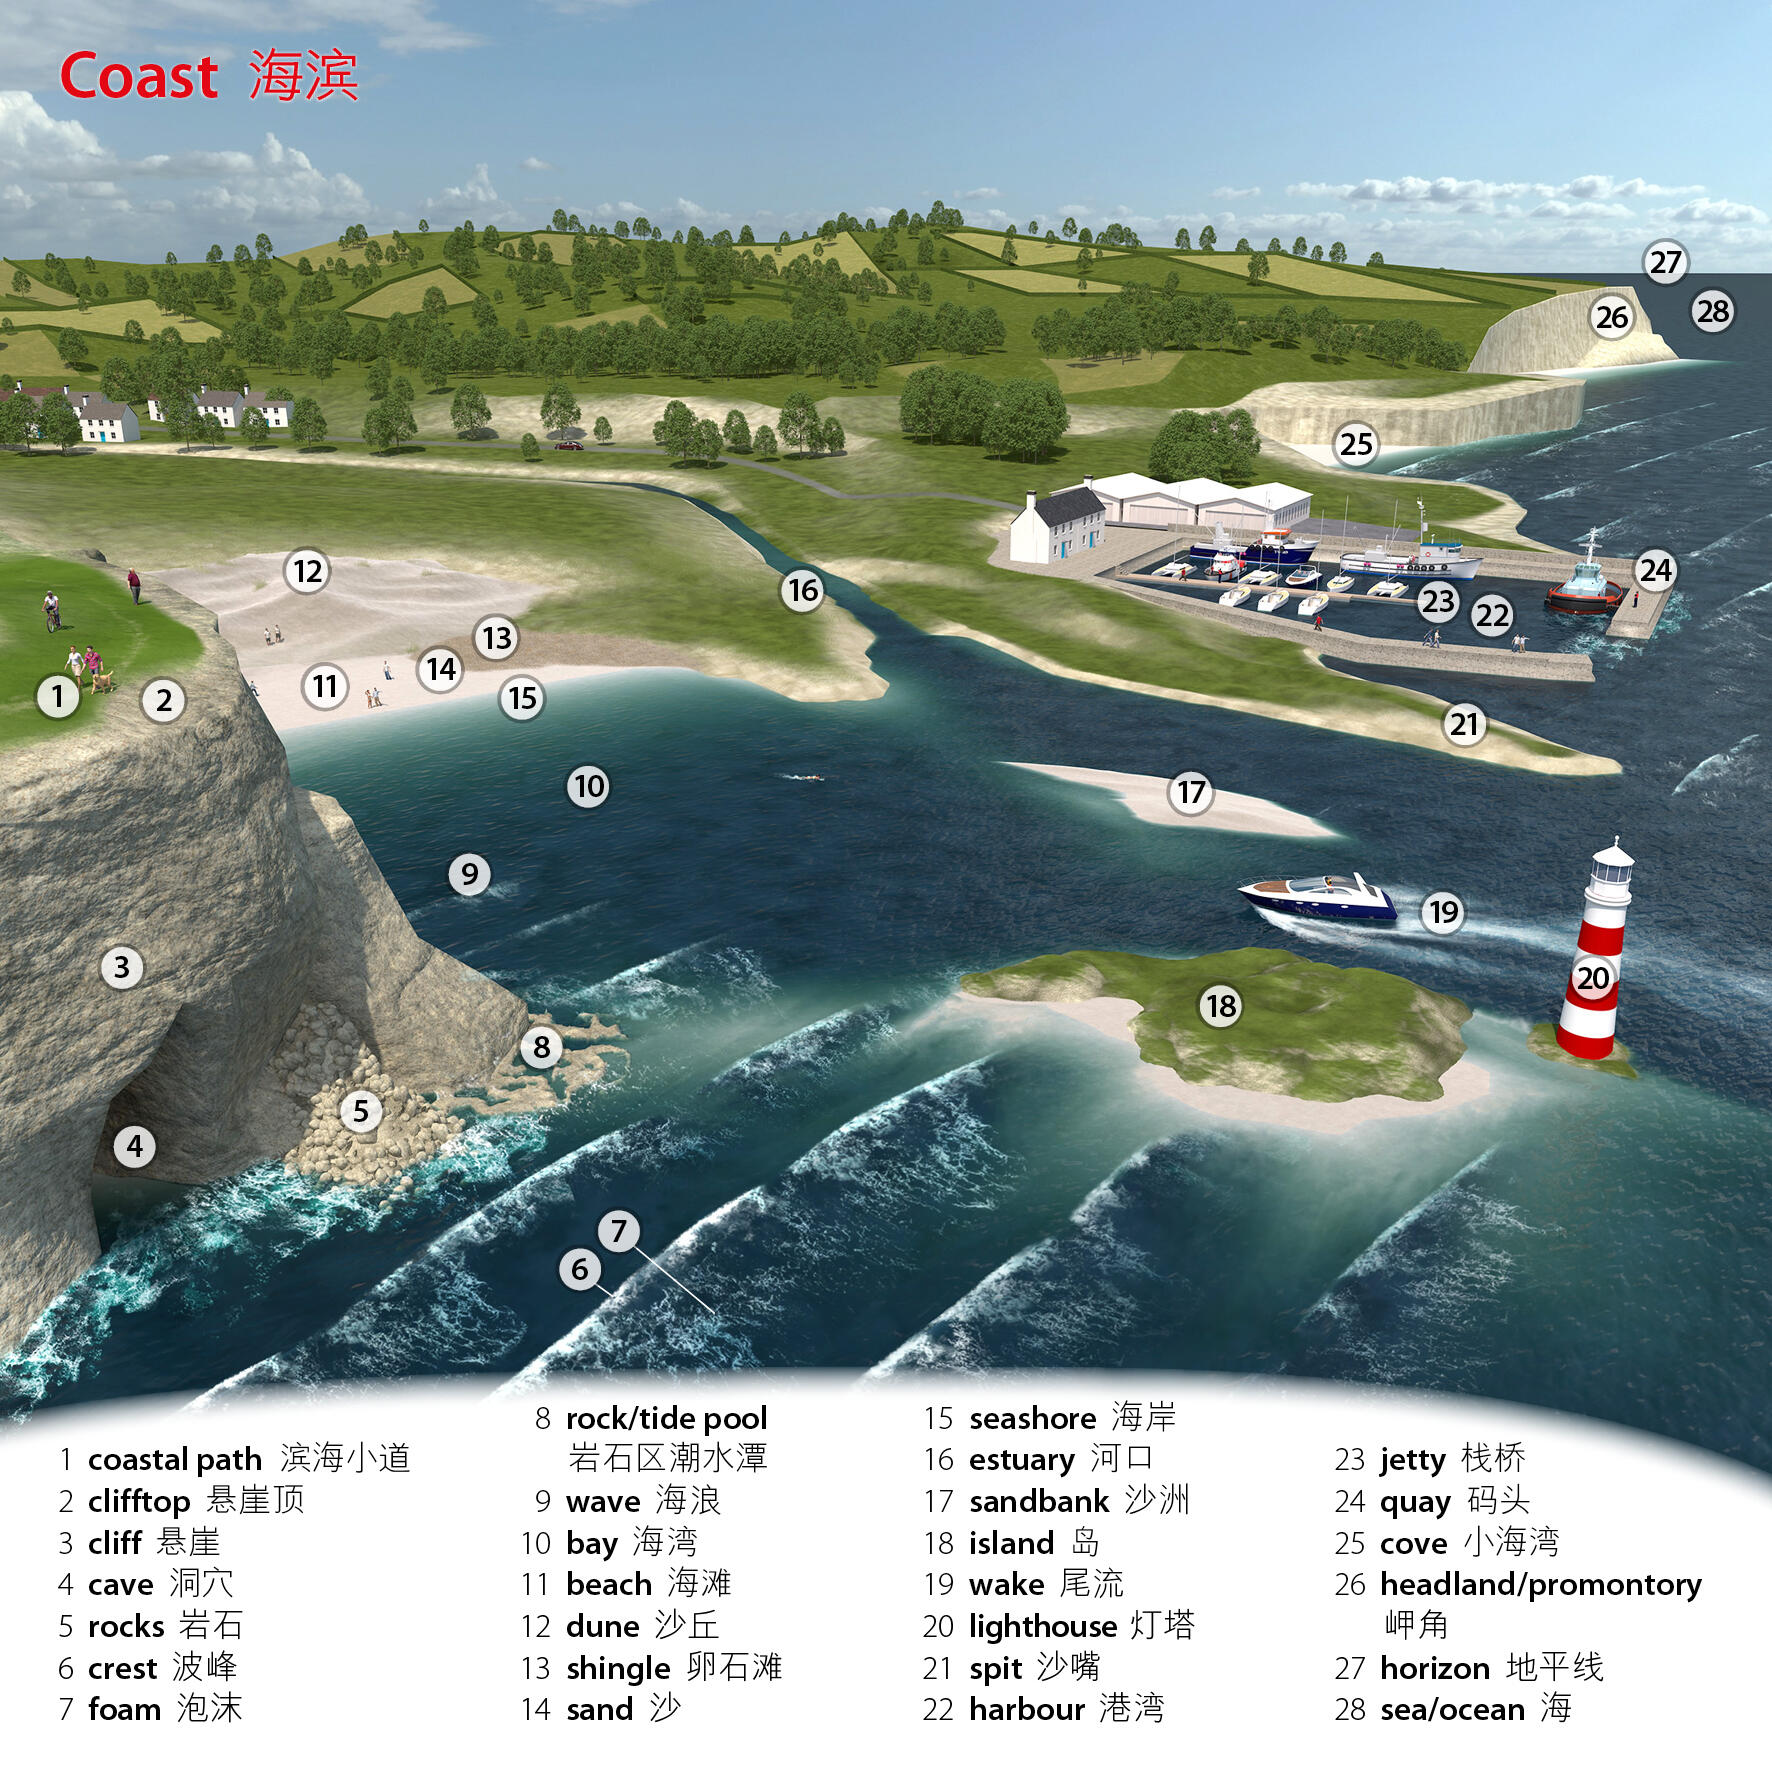
\includegraphics[width=0.82\textwidth]{fish/coast.png}
  \caption{\label{fig:coast}海滨各部分图例}
\end{figure}
\clearpage

鱼类介绍有参考豆瓣cocojamboo文章

\url{https://book.douban.com/subject/1064275/discussion/616533832/}

\dingphotoh{marlin}{marlin, 枪鱼,马林鱼}{老人捕获的马林鱼身长十八尺
  (5.48米),体重一千五百磅(680公斤)}{tuna}{tuna, 金枪鱼}{活跃而敏捷的食肉
  动物,拥有光滑的流线型身体,也是游动速度最快的远洋鱼类之一。}

\dingphotoh{dolphin}{dolphin, 鲯鳅}{体较大且延长侧扁,前部高大,向后渐变细。
  头大,背部很窄,成鱼头背几呈方形,额部有一骨质隆起,随成长而越明显,尤以雄
  鱼为甚。}{flying}{flying fish, 飞鱼}{体态修长,稍稍侧扁,长度一般为45厘米。
  吻短,口小,眼大。胸鳍发达如翼,腹鳍也比较发达。借由尾部迅速摆动,可达到极大
  的速度,然后跃出水面,张开胸鳍,可滑行百米以上的距离。}


\dingphotoh{Makoshark}{Mako shark, 鲭鲨}{老人碰见和杀死的第一条鲨鱼。身体光滑
  细长,鼻端呈长锥形。它的胸鳍很短,尾鳍呈半月形。尾巴底部有明显的龙骨。牙齿
  幼长及轻微弯曲,当嘴巴紧合时仍可看见牙齿。雌鲨成年体长约2米,雄鲨成年体长
  约1.3米,最大体型约3.7米。 }{galanos}{galanos, 西班牙语中一种鲨鱼,可能
  是“直翅真鲨”}{细长、流线型身体,吻部宽而圆,前鼻瓣不明显,眼睛是圆形的,
  中等大小,双颚两侧各有14排牙齿,其最长可达3.0米(9.8英尺),体重可达85.5公
  斤,寿命可达24年。}

\dingphotoh{heming1}{1933年,欧内斯特·海明威、卡洛斯·古铁雷斯、乔·拉塞尔和
  乔·洛与马林鱼}{}{heming2}{1934年,欧内斯特·海明威和卡洛斯·古铁雷斯驾驶皮
  拉尔号}{}

\dingphotoh{heming3}{1935年7月,波林·海明威、欧内斯特·海明威和他的三个
  儿子,与四条蓝色马林鱼}{}{heming4}{古巴渔民成功捕获鲨鱼}{}

\begin{figure}[ht!]
  \centering
  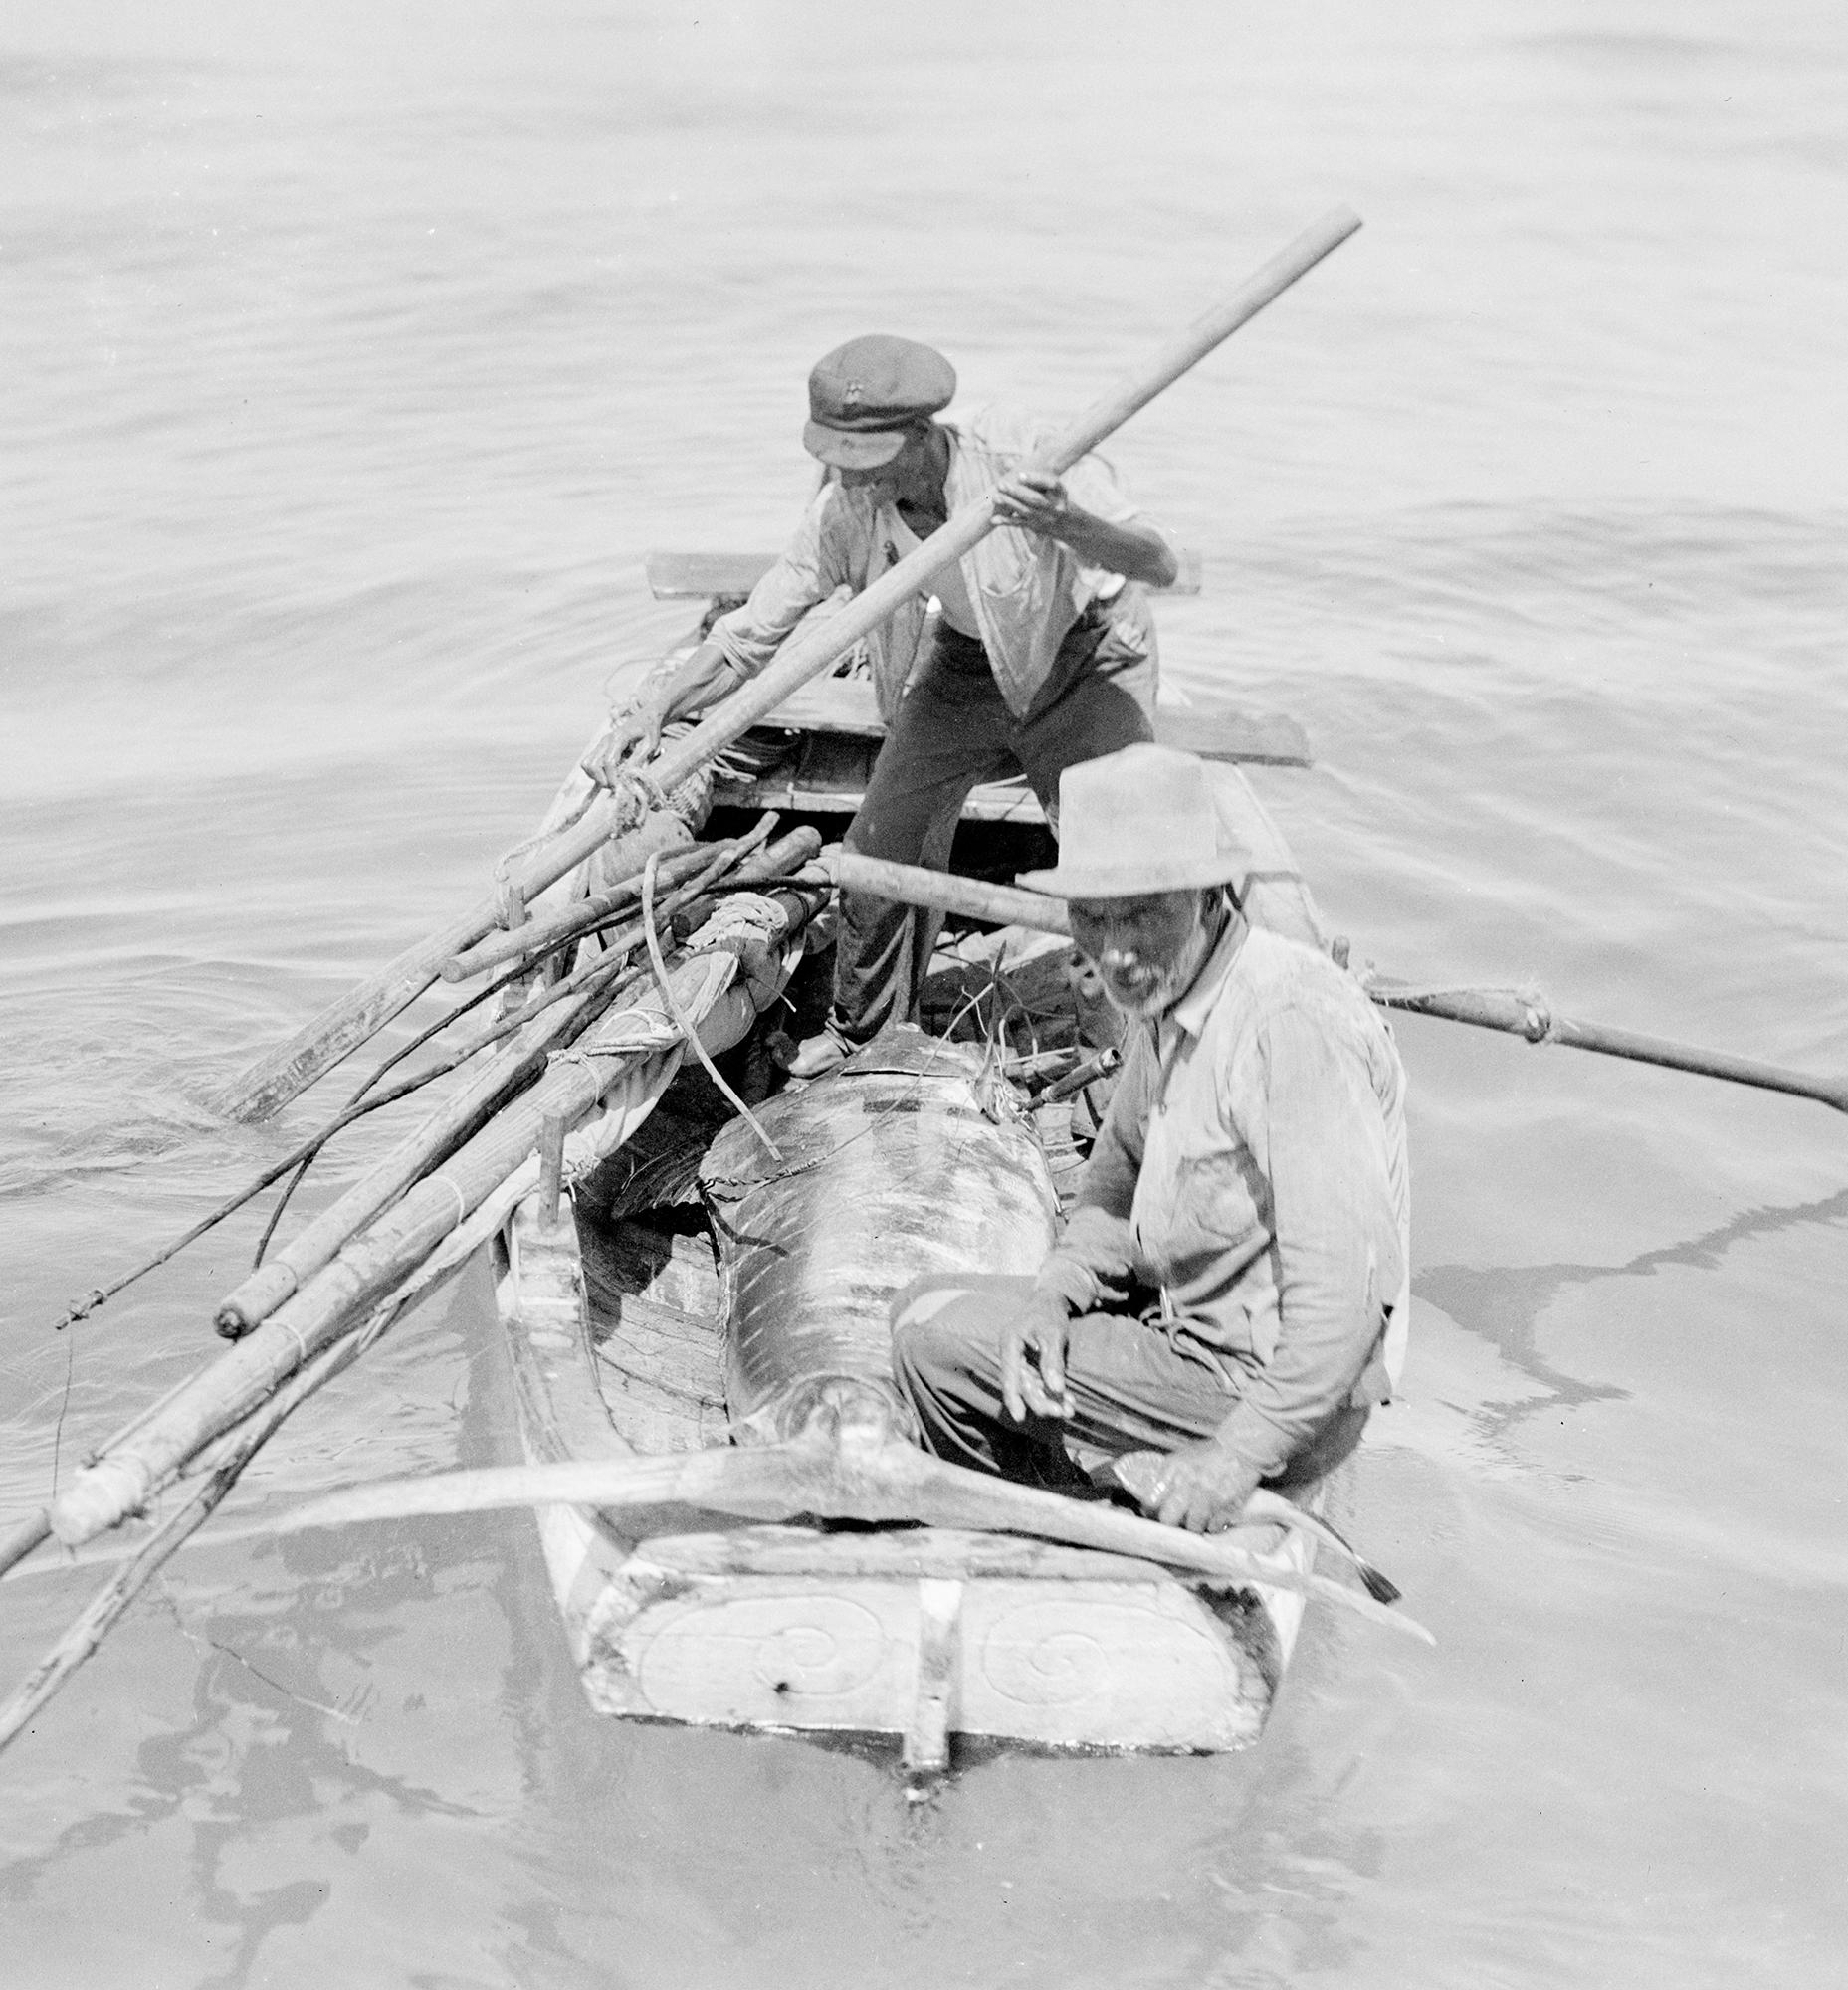
\includegraphics[width=0.95\textwidth]{fish/heming5.jpg} \caption{\label{fig:heming5}1955年,古巴科伊马尔的渔民带回了一条马林鱼}
\end{figure}

\chapter{The Old Man and the Sea}

He was an old man who fished alone in a \gls{skiff} in \uline{the \Gls{gulf}
  \Gls{stream}}\footnote{墨西哥湾} and he had gone eighty-four days now without
taking a fish. In the first forty days a boy had been with him. But after
forty days without a fish the boy's parents had told him that the old man
was now \gls{definitely} and finally \emph{salao}\footnote{源自西班牙
  语salado,原意是加了盐的,咸苦的,引申为倒霉的、不吉利的}, which is
\uline{the worst \gls{form} of unlucky}\footnote{字面意思是最坏的不幸类型,十足
  不幸的意思}, and the boy had gone \uline{at their orders}\footnote{听从他们
  (父母)的命令} in another boat which caught three good fish the first
week. It made the boy sad to see the old man come in each day with his
skiff empty and he always went down to help him carry \uline{either} the
\gls{coiled} lines \uline{or}\footnote{either \ldots{} or, 或者……或者……,要
  么……要么……} the \gls{gaff} and \gls{harpoon} and the \gls{sail} that was
\gls{furled} around the \gls{mast}. The sail was patched with \gls{flour}
\glspl{sack} and, \gls{furled}, it looked like the flag of \gls{permanent} \gls{defeat}.

The old man was thin and \gls{gaunt} with deep \glspl{wrinkle} in the back
of his neck. The brown \glspl{blotch} of the \gls{benevolent} \gls{skin}
cancer \uline{the sun \glspl{bring} from its \gls{reflection} on the
  \gls{tropic} sea}\footnote{前面省略了关系代词that。本从句修饰blotch} were
on his \glspl{cheek}. The blotches ran well down the sides of his face and his
hands had the \gls{deep-creased} \glspl{scar} from handling heavy fish on
the \glspl{cord}. But none of these scars were fresh. They were \gls{as} old
as \glspl{erosion} in a fishless desert\footnote{无鱼沙漠中的侵蚀。将伤疤与无
  鱼沙漠侵蚀联系在一起。无鱼沙漠对应捕鱼人的境遇,突出其凄凉。}.

Everything about him was old \gls{except} his eyes and they were the same
color as the sea and were \gls{cheerful} and \gls{undefeated}.

``Santiago,'' the boy said to him as they climbed the \gls{bank} from where the
skiff was \gls{hauled} up. ``I could go with you again. We've made some money.''

The old man had taught the boy to fish and the boy loved him.

``No,'' the old man said. ``You're with a lucky boat. Stay with them.''

``But remember how you went eighty-seven days without fish and then we caught big ones every day for three weeks.''

``I remember,'' the old man said. ``I know you did not leave me because you
\gls{doubted}.''\footnote{同样文字,不同语调节奏,会使句子产生不一样的含义,
  各国语言皆是。尝试用不同语调节奏朗读本句并且表露不同意思。}

``It was papa made me leave. I am a boy and I must \gls{obey} him.''

``I know,'' the old man said. ``It is quite normal.''

``He hasn't much \gls{faith}.''

``No,'' the old man said. ``But we have. Haven't we?''

``Yes,'' the boy said. ``Can I offer you a beer on the \gls{Terrace} and then we'll take the \gls{stuff} home.''

``Why not?'' the old man said. ``Between fishermen.''

They sat on the Terrace and many of the fishermen \uline{made fun
  of}\footnote{make fun of, 取笑,嘲弄} the old man and he was not angry.
Others, of the older fishermen, looked at him and were sad. But they did not
show it and they spoke \gls{politely} about the \gls{current} and the
\glspl{depth} they had \gls{drifted} their lines at and the \gls{steady}
good weather and of what they had seen.\footnote{其他老渔夫们所谈四件事均是为
  暖老人心。} The successful fishermen of that day were already in and had
\gls{butchered} their \gls{marlin} out and carried them \gls{laid} full
length across two \glspl{plank}, with two men \gls{staggering} \uline{at the
  end of} each plank, to the fish house where they waited for the ice truck
to carry them to the market in Havana. \uline{Those who had caught
  \glspl{shark}} had taken them to the shark factory on the other side of
the \gls{cove} where they were \gls{hoisted} on a \gls{block} and
\gls{tackle}, their \glspl{liver} removed, their \glspl{fin} cut off and
their \glspl{hide} \gls{skinned} out and their \gls{flesh} cut into
\glspl{strip} for salting.

When the wind was in the east a smell came across the \gls{harbour} from the
shark factory; but today there was only the \gls{faint} \gls{edge} of the
\gls{odour} because the wind had backed into the north and then \gls{drop_off}
and it was \gls{pleasant} and sunny on the Terrace.

``Santiago,'' the boy said.

``Yes,'' the old man said. He was holding his glass and \uline{thinking of}
many years ago.

``Can I go out to get \glspl{sardine} for you for tomorrow?''

``No. Go and play baseball. I can \gls{still} \gls{row} and Rogelio will \gls{throw} the net.''

``I would like to go. If I cannot fish with you. I would like to \gls{serve} in some way.''

``You bought me a beer,'' the old man said. ``You are already a man.''

``How old was I when you first took me in a boat?''

``Five and you nearly were killed when I brought the fish \uline{in too
  green}\footnote{字面意思“太绿了”。渔民俚语,形容被钓到的鱼没有被耗尽力气,
  还有太多活力。} and he\footnote{本书中,往往用he来指代大鱼,表示大鱼的雄性阳
  刚力量及其与渔民的特殊感情。} nearly \gls{tore} the boat to pieces. Can
you remember?''

``I can remember the tail \gls{slapping} and \gls{banging} and the \gls{thwart}
breaking and the noise of the \gls{clubbing}. I can remember you throwing me into
the \gls{bow} where the wet coiled lines were and feeling the whole boat \gls{shiver}
and the noise of you \gls{clubbing} him like \gls{chopping} a tree down and the \gls{sweet}
blood smell all \gls{over} me.''

``Can you really remember that or did I just tell it to you?''

``I remember everything from \uline{when we first went together}.''

The old man looked at him with his sun-burned, \gls{confident} loving eyes.

``If you were my boy I'd take you out and \gls{gamble},'' he said. ``But you are your father's and your mother's and you are in a lucky boat.''

``May I get the sardines? I know where I can get four \glspl{bait} too.''

``I have mine left from today. I put them in salt in the box.''

``Let me get four fresh ones.''

``One,'' the old man said. His hope and his \gls{confidence} had never gone. But now they were \gls{freshening} as when the \gls{breeze} \glspl{rise}.

``Two,'' the boy said.

``Two,'' the old man agreed. ``You didn't \gls{steal} them?''

``I would,'' the boy said. ``But I bought these.''

``Thank you,'' the old man said. He was \uline{too} simple \uline{to}
\gls{wonder} when he had \gls{attained} \gls{humility}. But he knew he had
attained it and he knew it was not \gls{disgraceful} and it carried no loss
of true \gls{pride}.

``Tomorrow is going to be a good day with this current,'' he said.

``Where are you going?'' the boy asked.

``Far out \uline{to come in when the wind \glspl{shift}}. I want to be out before it is light.''

``I'll try to get him to work far out,'' the boy said. ``Then if you \gls{hook} something truly big we can come to your \gls{aid}.''

``He does not like to work too far out.''

``No,'' the boy said. ``But I will see something that he cannot see such as a bird working and get him to come out after \gls{dolphin}.''

``Are his eyes that bad?''

``He is almost blind.''

``It is strange,'' the old man said. ``He never went \gls{turtle}-ing. That is what kills the eyes.''

``But you went turtle-ing for years off the Mosquito
Coast\footnote{\doulos{mɒsˈkiː.təʊ kəʊst},莫斯基托海岸} and your eyes
are good.''

``I am a \gls{strange} old man''

``But are you strong enough now for a truly big fish?''

``I think so. And there are many \glspl{trick}.''

``Let us take the \gls{stuff} home,'' the boy said. ``So I can get the \gls{cast} net and go after the sardines.''

They picked up the \gls{gear} from the boat. The old man carried the mast on
his \gls{shoulder} and the boy carried the wooden boat with the coiled,
hard-\gls{braided}\footnote{复合词。hard在这里作“坚实的,牢固的”。因为名词
  短语前置修饰语部分中,一个修饰成分只能是单个词,所以将两词用 hyphen - 连接
  复合。“牢固编织的”} brown lines, the gaff and the harpoon with its
\gls{shaft}. The box with the baits was under the \gls{stern} of the
skiff along with the club that was used to \gls{subdue} the big fish
when they were brought \gls{alongside}. No one would \gls{steal} from the
old man but it was better to take the sail and the heavy lines home \uline{as
the \gls{dew} was bad for them} and, though he was quite sure no local people
would steal from him, the old man thought that a gaff and a harpoon were
\gls{needless} \glspl{temptation} to leave in a boat.

They walked up the road together to the old man's \gls{shack} and
\uline{went in} \uline{through its open door}. The old man \gls{leaned} the
mast with its \gls{wrapped} sail \gls{against} the wall and the boy put the
box and the other gear beside it. The mast was \gls{nearly} \uline{as long
  as}\footnote{\textbf{as long as: 一直;像……一样长;只要。}} the one
room of the shack. The shack was made of the \gls{tough} \glspl{budshield}
of the \gls{royal_palm} which are called \emph{guano}\footnote{royal palm的西
  班牙语。} and in it there was a bed, a table, one chair, and a place on
the dirt floor to cook with \gls{charcoal}. On the brown walls of the
\gls{flattened}, \gls{overlapping} leaves of the \gls{sturdy} \gls{fibered}
\emph{guano} there was a \gls{picture} in color of the Sacred Heart of
Jesus\footnote{耶稣圣心图} and another of the Virgin of Cobre\footnote{科布莱
  圣母图}. These were \glspl{relic} of his wife. Once there had been a
\gls{tinted} photograph of his wife on the wall but he had taken it down
because it made him \uline{too} lonely \uline{to} see it and it was on the
shelf in the corner \uline{under his clean shirt}.\footnote{这句建议细加品味。}

``What do you have to eat?'' the boy asked.

``A \gls{pot} of yellow rice with fish. Do you want some?''

``No. I will eat at home. Do you want me to make the fire?''

``No. I will make it later on. Or I may eat the rice cold.''

``May I take the cast net?''

``Of course.''

There was no cast net and the boy remembered when they had sold
it\footnote{when they had sold it 名词性关系从句}. But they went through
this \gls{fiction} every day. There was no pot of yellow rice and fish and the boy
knew this too.\footnote{This sentence is sad yet heartwarming.}

``Eighty-five is a lucky number,'' the old man said. ``How would you like to
see me bring one in that \gls{dressed_out} over a thousand \glspl{pound}\footnote{that关系
  子句的先行词是one。被需结合紧密的bring \ldots{} in(带来,介入;挣到)中
  的in挤出到后面。}?''

``I'll get the cast net and go for sardines. Will you sit in the sun in the \gls{doorway}?''

``Yes. I have yesterday's paper and I will read the baseball.''

The boy did not know whether yesterday's paper was a fiction too. But the
old man brought it out \uline{from under the bed}.

``Perico gave it to me at the \emph{bodega}\footnote{bodega, \doulos{bәʊˈdiːɡә},
  西班牙语“酒店”。},'' he explained.

``I'll be back when I have the sardines. I'll keep yours and mine together
on ice and we can share them in the morning. When I come back you can tell
me about the baseball.''

``The Yankees\footnote{纽约扬基棒球队} cannot lose.''

``But I fear the Indians of Cleveland\footnote{克利夫兰印第安人队}.''

``Have faith in the Yankees my son. Think of the great DiMaggio.''

``I fear both the Tigers of Detroit\footnote{底特律老虎队} and the Indians of Cleveland.''

``Be careful or you will fear even the Reds of Cincinnati and the White Sax of Chicago\footnote{辛辛那提红队和芝加哥白袜队}.''

``You study it and tell me when I come back.''

``Do you think we should buy a \gls{terminal} of the lottery with an eighty-five?
Tomorrow is the eighty-fifth day.''

``We can do that,'' the boy said. ``But what about the eighty-seven of your great record?''

``It could not happen twice. Do you think you can find an eighty-five?''

``I can \gls{order} one.''

``One sheet. That's two dollars and a half. Who can we borrow that from?''

``That's easy. I can always borrow two dollars and a half.''

``I think perhaps I can too. But I try not to borrow\footnote{not否定的不是整
  个句子,而是try之后部分。}. First you borrow. Then you beg.''

``Keep warm old man,'' the boy said. ``Remember we are in September.''

``The month \uline{when the great fish come}\footnote{状语关系从句},'' the old
man said. ``Anyone can be a fisherman in May.''

``I go now for the sardines,'' the boy said.

When the boy came back the old man was \gls{asleep} in the chair and the sun was
down. The boy took the old army \gls{blanket} off the bed and \gls{spread}
it over the back of the chair and over the old man's shoulders. They were
strange shoulders, still powerful although very old, and the neck was still
strong too and the \glspl{crease} did not show so much when the old man was
asleep and his head fallen forward. His shirt had been \gls{patched} so many
times that it was like the sail and the patches were \gls{faded} to many
different \glspl{shade} by the sun. The old man's head was very old though
and with his eyes closed there was no life in his face. The newspaper
\gls{lay} across his \glspl{knee} and the weight of his arm held it there in
the evening breeze. He was \gls{barefooted}.

The boy left him there and when he came back the old man was still asleep.

``Wake up old man,'' the boy said and put his hand on one of the old man's
knees.

The old man opened his eyes and for a moment he was coming back \uline{from
  a long way away}. Then he smiled.

``What have you got?'' he asked.

``Supper,'' said the boy. ``We're going to have supper.''

``I'm not very hungry.''

``Come on and eat. You can't fish and not eat.''

``I have,'' the old man said getting up and taking the newspaper and \gls{folding} it. Then he started to fold the blanket.

``Keep the blanket around you,'' the boy said. ``\uline{You'll not fish without
eating while I'm alive.}''

``Then live a long time and take care of yourself,'' the old man said. ``What are we eating?''

``Black beans and rice, \gls{fried} bananas, and some \gls{stew}.''

The boy had brought them in a two\gls{-decker} metal container from the
Terrace. The two \gls{sets} of knives and forks and \glspl{spoon} were in his pocket with
a paper \gls{napkin} wrapped around each set.

``Who gave this to you?''

``Martin. The owner.''

``I must thank him.''

``I thanked him already,'' the boy said. ``You don't need to thank him.''

``I'll give him the \gls{belly} meat of a big fish,'' the old man said. ``Has he done this for us more than once?''

``I think so.''

``I must give him something more than the belly meat then. He is very \gls{thoughtful} for us.''

``He sent two beers.''

``I like the beer in \glspl{can} best.''

``I know. But this is in bottles, Hatuey beer, and I take back the bottles.''

``That\uline{'s very kind of} you,'' the old man said. ``Should we eat?''

``I've been asking you to,'' the boy told him gently. ``I have not wished to open the container until you were ready.''

``I'm ready now,'' the old man said. ``I only needed time to wash.''

Where did you wash? the boy thought. The village water \gls{supply} was
\uline{two streets down the road}\footnote{沿着这条路走两条街。}. I must have water here for him, the boy
thought, and \gls{soap} and a good \gls{towel}. Why am I so
\gls{thoughtless}? I must get him another shirt and a jacket for the winter
and some \uline{sort of} shoes and another blanket.

``Your stew is excellent,'' the old man said.

``Tell me about the baseball,'' the boy asked him.

``In the American \Gls{league} it is the Yankees as I said,'' the old man said happily.''

``They lost today,'' the boy told him.

``That means nothing. \uline{The great DiMaggio is himself again.}''

``They have other men on the team.''

``\Gls{naturally}. But he makes the difference. In the other league,
\uline{between} Brooklyn \uline{and} Philadelphia I must take Brooklyn. But
then I think of Dick Sisler and those great drives in the old park.''

``There was nothing ever like them. He hits the longest ball I have ever seen.''

``Do you remember \uline{when he used to come to the Terrace}\footnote{名词性
  疑问从句}? I wanted to take him fishing but I was \uline{too} \gls{timid}
\uline{to} ask him. Then I asked you to ask him and you were too timid.''

``I know. It was a great \gls{mistake}. He might have gone with us. Then we
would have that for all of our lives.''

``I would like to take the great DiMaggio fishing,'' the old man said.
``They say his father was a fisherman. Maybe he was as poor as we are and
would understand.''

``The great Sisler's father was never poor and he, the father, was playing
in the Big Leagues \uline{when he was my age}.''

``When I was your age I was before the mast on a \gls{square}
  \gls{rigged} ship\footnote{方帆船。} that ran to Africa and I have seen
lions on the beaches in the evening.''

``I know. You told me.''

``Should we talk about Africa or about baseball?''

``Baseball I think,'' the boy said. ``Tell me about the great John J. McGraw.'' He said Jota for J.

``He \uline{used to} come to the Terrace sometimes too in the older days. But
he was \gls{rough} and \gls{harsh}-\gls{spoken} and difficult when he was
drinking. His mind was on \glspl{horse} as well as baseball. \Gls{at_least}
he carried lists of horses at all times in his pocket and \gls{frequently}
spoke the names of horses on the telephone.''

``He was a great manager,'' the boy said. ``My father \uline{thinks he was the greatest}.''

``Because he came here the most times,'' the old man said. ``If Durocher had
continued to come here each year your father would \uline{think him the
  greatest manager}\footnote{试比较本句与上句thinks he was the greatest的区别。}.''

``Who is the greatest manager, really, Luque or Mike Gonzalez?''

``I think they are \gls{equal}.''

``And the best fisherman is you.''

``No. I know others better.''

``\emph{Qué Va}\footnote{西班牙语,“干嘛这么说”},'' the boy said. ``There are
many good fishermen and some great ones. But there is only you.''

``Thank you. You make me happy. I hope no fish will \gls{come_along} so great that
he will prove us wrong.\footnote{我希望不会出现一条太大的鱼以证明我们是错的。}''

``There is no such fish if you are still strong as you say.''

``I may not be as strong as I think,'' the old man said. ``But I know many tricks and I have \gls{resolution}.''

``You \uline{ought to} go to bed now so that you will be \gls{fresh} in the
morning. I will take the things back to the Terrace.''

``Good night then. I will wake you in the morning.''

``You're my alarm clock,'' the boy said.

\textbf{``Age is my alarm clock,'' the old man said. ``Why do old men wake
  so early? Is it to have one longer day?''}\footnote{\textbf{be to do sth,
    将要做某事。be to do with sb/sth, 与某人或某事有关。be to相当于半情态助动
    词。}}

``I don't know,'' the boy said. ``All I know is that young boys sleep late and hard.''

``I can remember it,'' the old man said. ``I'll \gls{waken} you \uline{in
  time}\footnote{\textbf{in time, 及时;迟早,最终。on time, 准时,按时。at times, 有时,偶尔。}}.''

``I do not like \uline{for him to waken me}\footnote{for sb to do sth, 其中
  sb是后面不定式的逻辑主语!}. It is \gls{as_though} I were \gls{inferior}.''

``I know.''

``Sleep well old man.''

The boy went out. They had eaten with no light on the table and the old man
took off his trousers and went to bed in the dark. He \gls{rolled} his
trousers up to make a \gls{pillow}, putting the newspaper inside them. He
rolled himself in the blanket and slept on the other old newspapers that
covered the springs\footnote{语言比语法更有活力。英语spring与汉语“春天”
  同样有“朝气,活力”的意思。} of the bed.

He was asleep in a short time and he dreamed of \gls{Africa} when he was a
boy and the long golden beaches and the white beaches, so white they hurt
your eyes, and the high capes and the great brown mountains. He lived along
that coast now every night and in his dreams he heard the \gls{surf}
\gls{roar} and saw the \gls{native} boats come riding through it. He smelled
the \gls{tar} and \gls{oakum} of the \gls{deck} as he slept and he smelled
the smell of Africa that the land breeze brought at morning.

Usually when he smelled the land breeze he woke up and dressed to go and
wake the boy. But tonight the smell of the land breeze came very early and
he knew it was too early in his dream and went on\footnote{go on, 继续,坚
  持。} dreaming to see the white \glspl{peak} of the
Islands\footnote{Islands, 首字母大写,古巴附近某个群岛专有名词的缩写。} rising from
the sea and then he dreamed of the different harbours and roadsteads of the
Canary Islands.

\textbf{He no longer dreamed of storms, nor of women, nor of great
  \glspl{occurrence}, nor of great fish, nor fights, nor contests of
  \gls{strength}, nor of his wife. He only dreamed of places now and of the
  lions on the beach.}\footnote{nor of和 nor展示语调情绪的变化。} They
played like young cats in the \gls{dusk} and he loved them as he loved the boy. He
never dreamed about the boy. He simply woke, looked out the open door at the
moon and unrolled his trousers and put them on. He \gls{urinated} outside
the shack and then went up the road to wake the boy. He was shivering with
the morning cold. But he knew he would shiver himself warm and that soon he
would be rowing.

The door of the house where the boy lived was unlocked and he opened it and
walked in quietly with his \gls{bare} \gls{feet}. The boy was asleep on a
\gls{cot} in the first room and the old man could see him clearly with
\uline{the light that came in from the dying moon}. He took hold of one foot
\gls{gently} and held it until the boy woke and turned and looked at him.
The old man \gls{nodded} and the boy took his trousers from the chair by the
bed and, sitting on the bed, pulled them on.

The old man went out the door and the boy came after him. He was sleepy and
the old man put his arm across his shoulders and said, ``I am \gls{sorry}.''

``\emph{Qué Va},'' the boy said. ``It is what a man must do.''

They walked down the road to the old man's shack and all along the road, in
the dark, barefoot men were moving, carrying the masts of their boats.

When they \gls{reached} the old man's shack the boy took the rolls of line
in the basket and the harpoon and gaff and the old man carried the mast with
the furled sail on his shoulder.

``Do you want coffee?'' the boy asked.

``We'll put the gear in the boat and then get some.''

They had coffee from \gls{condensed} milk cans at an early morning place that served fishermen.

``How did you sleep old man?'' the boy asked. He was waking up now \gls{although}
it was still hard for him to leave his sleep.

``Very well, Manolin,'' the old man said. ``I feel confident today.''

``So do I,'' the boy said. ``Now I must get your sardines and mine and your
fresh baits. He brings our gear himself. He never wants anyone to carry
anything.''

``We're different,'' the old man said. ``I let you carry things when you were five years old.''

``I know it,'' the boy said. ``I'll be right back. Have another coffee. We have \gls{credit} here.''

He walked off, bare-footed on the \gls{coral} rocks, to the ice house where
the baits were stored.

The old man drank his coffee slowly. It was all he would have all day and he
knew that he should take it. For a long time now eating had bored him and he
never carried a lunch. He had a bottle of water in the bow of the
skiff and that was all he needed for the day.

The boy was back now with the sardines and the two baits wrapped in a
newspaper and they went down the \gls{trail} to the skiff, feeling the
\gls{pebbled} sand under their feet, and \gls{lifted} the skiff and
\gls{slid} her into the water.

``Good luck old man.''

``Good luck,'' the old man said. He fitted the rope \glspl{lashing} of the
\glspl{oar} onto the \gls{thole}
\glspl{pin} and, \gls{leaning} forward against the \gls{thrust} of the
\glspl{blade} in the water, he began to row out of the harbour in the dark.
There were other boats from the other beaches going out to sea and the old
man heard the \uline{\gls{dip} and push} of their oars even though he could
not see them now the moon was below the hills.

Sometimes someone would speak in a boat. But most of the boats were silent
except for the \gls{dip} of the oars. They spread \gls{apart} after they
were out of the mouth of the harbour and each one headed for the part of the
ocean where he hoped to find fish. The old man knew he was going far out and
he left the smell of the land behind and rowed out into \uline{the clean
  early morning smell of the ocean}. He saw the \gls{phosphorescence} of the
Gulf weed in the water as he rowed over the part of the ocean that the
fishermen called the great well\footnote{此处well为名词,“井,水井,油井,天
  然气井,电梯井等。”} because there was a \gls{sudden} deep of seven
hundred \glspl{fathom} where all sorts of fish \gls{congregated} because of
\uline{the \gls{swirl}} \uline{the current made against the \gls{steep}
  walls of the floor of the ocean}. Here there were \glspl{concentration} of
\gls{shrimp} and bait fish and sometimes \glspl{school} of \gls{squid} in
the deepest holes and these \gls{rose} \gls{close_to} the \gls{surface} at
night where all the \gls{wandering} fish fed on them\footnote{fed on them, 以
  他们为食。fed, feed的过去式,喂养,饲养。}.

In the dark the old man could feel the morning coming and as he rowed he
heard the \gls{trembling} sound as flying fish left the water and the
\gls{hissing} that their \gls{stiff} set \glspl{wing} made as they
\gls{soared} away in the darkness. He was very \gls{fond} of flying fish as
they were his \gls{principal} friends on the ocean. He was \gls{sorry} for
the birds, especially the small \gls{delicate} dark \glspl{tern} that were
always flying and looking and almost never finding, and he thought, ``the
birds have a harder life than we do except for the \gls{robber} birds and
the heavy strong ones. Why did they make birds so delicate and fine as those
sea \glspl{swallow} when\footnote{这里的when是 “in view of the fact that;
  considering that: 既然;考虑到”的意思,不是“什么时候”。} the ocean can
be so \gls{cruel}? She\footnote{大海和船只在渔民眼中往往是女性的。} is kind and very beautiful. But she can be so cruel
and it comes so suddenly and such birds that fly, dipping and
\gls{hunting},\footnote{夹在两个逗号中间的dipping and hunting是非限制性修饰语,
  修饰such birds that fly.} with their small sad voices are made too
\gls{delicately} for the sea.''

He always thought of the sea as \emph{la mar}\footnote{西班牙语,mar是“海
  洋”,la是前面的阴性定冠词,而下文的el是阳性定冠词。} which is what people
call her in Spanish when they love her. Sometimes those who love her say bad
things of her but they are always said \uline{as though}\footnote{同as if,
  好像,似乎,仿佛。} she were a woman. Some of
the younger fishermen, those who used \glspl{buoy} as \glspl{float} for
their lines and had motorboats, bought when the shark livers had brought
much money, spoke of her as \emph{el mar} which is \gls{masculine}. They
spoke of her as a \gls{contestant} or a place or even an \gls{enemy}. But
the old man always thought of her as \gls{feminine} and as something that
gave or \gls{withheld} great \glspl{favour}, and if she did wild or
\gls{wicked} things it was because she could not help them. The moon
\glspl{affect} her as it does a woman, he thought.

He was rowing \gls{steadily} and it was no \gls{effort} for him since he kept well
within his speed and the surface of the ocean was flat except for the
\gls{occasional} swirls of the current. He was letting the current do \uline{a third of
the work}\footnote{三分之一的力气} and as it started to be light he saw he was already further out
than he had hoped to be at this hour.

I worked the deep wells for a week and did nothing, he thought. Today I'll
work out where the schools of \gls{bonito} and \gls{albacore} are and
\uline{maybe} there will be a big one with them.

Before it was really light he had his baits out and was \gls{drifting} with
the current. One bait was down forty fathoms. The second was at seventy-five
and the \uline{third and fourth} were down in the blue water at \uline{one hundred}
and \uline{one hundred and twenty-five} fathoms. Each bait \gls{hung} head
down with the \gls{shank} of the hook inside the bait fish, \gls{tied} and
\gls{sewed} \gls{solid} and all the \gls{projecting} part of the hook, the
\gls{curve} and the point, was covered with fresh sardines. Each sardine was
hooked through both eyes so that they made a half-\gls{garland} on the
projecting \gls{steel}. There was no part of the hook that a great fish
could feel which was not sweet smelling and good tasting.

The boy had given him two fresh small tunas, or albacores, which hung on the
two deepest lines like \glspl{plummet} and, on the others, he had a big blue
\gls{runner} and a yellow jack\footnote{blue runner, 金鲹鱼。yellow jack,巴
  氏若鲹鱼。} that had been used before; but they were in good
\gls{condition} still and had the \gls{excellent} sardines to give them
\gls{scent} and \gls{attractiveness}. Each line, as \gls{thick} around as a
big pencil, was looped onto a green-sapped \gls{stick}\footnote{a
  green-sapped stick, 绿干枝。sapped有一个较少用到的意思,to drain the sap
  from sth, 把树的汁液排干。老人用其作为“鱼漂”。} so that any pull or
touch on the bait would make the stick dip and each line had two
forty-fathom coils which could be made fast\footnote{这里的fast为副词,表
  示 ``securely attached/ firmly tied'' “牢固绑定,系牢地”。后文还会多次出
  现。} to the other \gls{spare} coils so that, if it were necessary, a fish
could take out over three hundred fathoms of line.

Now the man watched the dip of the three sticks over the side of the skiff
and rowed gently to keep the lines \gls{straight} up and down and at their \gls{proper}
depths. It was quite light and any moment now the sun would rise.

The sun rose \gls{thinly} from the sea and the old man could see the other boats,
low on the water and well in \gls{toward} the \gls{shore}, spread out across the
current. Then the sun was brighter and the \gls{glare} came on the water and
then, as it rose clear, the \gls{flat} sea sent it back at his eyes so that it
hurt \gls{sharply} and he rowed without looking into it. He looked down into the
water and watched the lines that went straight down into the dark of the
water. He kept them straighter than anyone did, so that at each level in
the darkness of the stream there would be a bait waiting exactly where he
wished it to be for any fish that swam there. Others let them drift with
the current and sometimes they were at sixty fathoms when the fishermen
thought they were at a hundred.

But, he thought, I keep them with \gls{precision}.\textbf{ Only I have no
  luck any more. But who knows? Maybe today. Every day is a new day. It is
  better to be lucky. But I would rather be exact. Then when luck comes you
  are ready.}

The sun was two hours higher now and it did not hurt his eyes so much to
look into the east. There were only three boats in \gls{sight} now and they
showed very low and far \gls{inshore}.

All my life the early sun has hurt my eyes, he thought. Yet they are still
good. In the evening I can look straight into it without getting the
blackness. It has more \gls{force} in the evening too. But in the morning it is
\gls{painful}.

Just then he saw a man-of-war bird\footnote{军舰鸟} with his long black
wings circling in the sky \gls{ahead} of him. He made a quick drop,
\gls{slanting} down on his back-swept wings, and then circled again.

``He's got something,'' the old man said aloud. ``He's not just looking.''

He rowed slowly and steadily toward where the bird was circling. He did not
hurry and he kept his lines straight up and down. But he \gls{crowded} the
current a little so that he was still fishing correctly \textbf{though}
\uline{faster} \textbf{than} \textbf{he would have fished if he was not trying
  to use the bird}.

The bird went higher in the air and circled again, his wings
\gls{motionless}. Then he \gls{dove} suddenly and the old man saw flying
fish \gls{spurt} out of the water and sail \gls{desperately} over the surface.

``Dolphin,'' the old man said aloud. ``Big dolphin.''

He shipped his oars\footnote{将桨搁入船内} and brought a small line from
under the bow. It had a \gls{wire} \gls{leader} and a medium-sized hook and
he baited it with one of the sardines. He let it go over the side and then
made it \uline{fast} to a ring \gls{bolt} in the stern. Then he baited
another line and left it coiled in the shade of the bow. He \uline{went back
  to rowing and to watching}\footnote{go back to中的to为介词,后接名词、代词
  或现在分词。} the long-winged black bird who was working, now, low over
the water.

As he watched the bird dipped again slanting his wings for the dive and then
\gls{swinging} them wildly and \gls{ineffectually} as he followed the flying fish.
The old man could see the \gls{slight} \gls{bulge} in the water that the big
dolphin raised as they followed the escaping fish. The dolphin were cutting
through the water below the flight of the fish and would be in the water,
driving at speed, when the fish dropped. It is a big school of dolphin, he
thought. They are \gls{widespread} and the flying fish have little
\gls{chance}. The bird has no chance. The flying fish are too big for him
and they go too fast.

He watched the flying fish \gls{burst} out again and again and the
\gls{ineffectual} movements of the bird. That school has gotten away from
me, he thought. They are moving out too fast and too far. But perhaps I will
pick up a \gls{stray} and perhaps my big fish is around them. My big fish must be
somewhere.

The clouds over the land now rose like mountains and the coast was only a
long green line with the gray blue hills behind it. The water was a dark
blue now, \uline{so} dark \uline{that} it was almost purple. As he \uline{looked down into it}
he saw the red sifting of the \gls{plankton} in the dark water and the
strange light the sun made now. He watched his lines to see them go straight
down out of sight into the water and he was happy to see so much plankton
because it \gls{meant} fish. The strange light the sun made in the water,
now that the sun was higher, meant good weather and so did the shape of the
clouds over the land. But the bird was almost out of sight now and nothing
showed on the surface of the water but some patches of yellow,
sun-\gls{bleached} \gls{Sargasso} \gls{weed} and the purple,
\gls{formalized}, \gls{iridescent}, \gls{gelatinous} \gls{bladder} of a
Portuguese man-of-war\footnote{葡萄牙僧帽水母,有致命剧毒。} floating close
beside the boat. It turned on its side and then righted itself. It floated
cheerfully as a \gls{bubble} with its long deadly purple \glspl{filament}
\gls{trailing} a \gls{yard} behind it in the water.

``\emph{Agua mala}\footnote{西班牙语,原意为"被败坏了的海水",因为水母的触须
  上有带有毒性的黏液 ,这里指毒水母。},'' the man said. ``You \gls{whore}.''

From where he \gls{swung} lightly against his oars he looked down into the
water and saw the tiny fish that were coloured like the trailing filaments
and swam between them and under the small shade the bubble made as it
drifted. They were \gls{immune} to its \gls{poison}. But men were not and
when same of the filaments would catch on a line and rest there \gls{slimy}
and purple while the old man was working a fish, he would have \glspl{welt}
and \glspl{sore} on his arms and hands of the sort that poison \gls{ivy} or poison
\gls{oak} can give. But these \glspl{poisoning} from the agua mala came quickly and
\gls{struck} like a \gls{whiplash}.

The iridescent bubbles were beautiful. But they were the \gls{falsest} thing
in the sea and the old man loved to see the big sea turtles eating
them. The turtles saw them, \gls{approached} them from the front, then shut
their eyes so they were completely \gls{carapaced} and ate them filaments
and all. The old man loved to see the turtles eat them and he loved to walk
on them on the beach after a storm and hear them pop when he stepped on them
with the \gls{horny} \glspl{sole} of his feet.

He loved green turtles and \glspl{hawksbill} with their \gls{elegance} and
speed and their great value and he had a friendly \gls{contempt} for the
huge, stupid \glspl{loggerhead}, yellow in their armour-plating, strange in their
love-making, and happily eating the Portuguese men-of-war with their eyes
shut.

He had no \gls{mysticism} about turtles although he had gone in turtle boats
for many years. He was sorry for them all, even the great \gls{trunk} \gls{backs}
that were \uline{as long as} the skiff and \gls{weighed} a ton. Most people are
\gls{heartless} about turtles because a turtle's heart will beat for hours
after he has been cut up and butchered. But the old man thought, I have such
a heart too and my feet and hands are like theirs. He ate the white eggs to
give himself strength. He ate them all through May to be strong in September
and October for the truly big fish.

He also drank a cup of shark liver oil each day from the big \gls{drum} in the
shack where many of the fishermen kept their gear. It was there for all
fishermen who wanted it. Most fishermen hated the taste. But it was no worse
than getting up at the hours that they rose and it was very good against all
colds and \gls{grippes} and it was good for the eyes.

Now the old man looked up and saw that the bird was circling again.

``He's found fish,'' he said aloud. No flying fish broke the surface and there
was no \gls{scattering} of bait fish. But as the old man watched, a small tuna
rose in the air, turned and dropped head first into the water. The tuna
\gls{shone} \gls{silver} in the sun and after he had dropped back into the water
\uline{another and another} rose and they were jumping in all \glspl{direction},
\gls{churning} the water and \gls{leaping} in long jumps after the bait. They
were circling it and driving it.

If they don't travel too fast I will get into them, the old man thought, and
he watched the school working the water white and the bird now dropping and
dipping into the bait fish that were forced to the surface in their \gls{panic}.

``The bird is a great help,'' the old man said. Just then the stern line
came \gls{taut} under his foot, where he had kept a loop of the line, and he
dropped his oars and felt the weight of the small tuna's shivering
\gls{pull} as he held the line firm and \gls{commenced} to \gls{haul} it in.
The shivering increased as he pulled in and he could see the blue back of
the fish in the water and the gold of his sides before he swung him over the
side and into the boat. He lay in the stern in the sun, \gls{compact} and
\gls{bullet} shaped, his big, \gls{unintelligent} eyes staring as he
\gls{thumped} his life out against the \gls{planking} of the boat with the
quick shivering \glspl{stroke} of his \gls{neat}, fast-moving tail. The old
man hit him on the head for \gls{kindness} and kicked him, his body still
\gls{shuddering}, under the shade of the stern.

``Albacore,'' he said aloud. ``He'll make a beautiful bait. He'll weigh ten pounds.''

He did not remember when he had first started to talk aloud when he was by
himself. He had \gls{sung} when he was by himself in the old days and he had
sung at night sometimes when he was alone steering \uline{on his
  watch}\footnote{on his watch, 在他值班时。} in the \glspl{smack} or in the
turtle boats. He had probably started to talk aloud, when alone, when the
boy had left. But he did not remember. When he and the boy fished together
they usually spoke only when it was necessary. They talked at night or when
they were \gls{storm-bound} by bad weather. It was \gls{considered} a
\gls{virtue} not to talk unnecessarily at sea and the old man had always
considered it so and respected it. But now he said his thoughts \gls{aloud}
many times since there was no one that they could \gls{annoy}.

``If the others heard me talking out loud they would think that I am
crazy,'' he said aloud. ``But since I am not crazy, I do not care. And the
rich have radios to talk to them in their boats and to bring them the
baseball.''

Now is no time to think of baseball, he thought. Now is the time to think of
only one thing. That which I was born for. There might be a big one around
that school, he thought. I picked up only a \gls{straggler} from the
albacore that were feeding. But they are working far out and fast.
\uline{Everything that shows on the surface today} travels very fast and to the
north-east. Can that be the time of day? Or is it some \gls{sign} of weather that
I do not know?

He could not see the green of the shore now but only the tops of the blue
hills that showed white \uline{as though} they were snow-\glspl{capped} and the
clouds that looked like high snow mountains above them. The sea was very
dark and the light made \glspl{prism} in the water. The \gls{myriad}
\glspl{fleck} of the plankton were \gls{annulled} now by the high sun and it
was only the great deep prisms in the blue water that the old man saw now
with his lines going straight down into the water that was a mile deep.

The tuna, the fishermen called all the fish of that \gls{species} tuna and
only \gls{distinguished} \gls{among} them by their proper names when they
came to sell them or to trade them for baits, were down again. The sun was
hot now and the old man felt it on the back of his neck and felt the \gls{sweat}
\gls{trickle} down his back as he rowed.

I could just drift, he thought, and sleep and put a \gls{bight} of line
around my \gls{toe} to wake me. But today is eighty-five days and I should
fish the day well.

Just then, watching his lines, he saw one of the projecting green
sticks dip sharply.

``Yes,'' he said. ``Yes,'' and shipped his oars without \gls{bumping} the
boat. He reached out for the line and held it softly between the \gls{thumb}
and \gls{forefinger} of his right hand. He felt \uline{no} \gls{strain}
\uline{nor} weight and he held the line lightly. Then it came again. This
time it was a \gls{tentative} pull, \uline{not} \gls{solid} \uline{nor}
heavy, and he knew exactly what it was. One hundred fathoms down a marlin
was eating the sardines that covered the point and the shank of the hook
where the hand-\gls{forged} hook projected from the head of the small tuna.

The old man held the line delicately, and softly, with his left hand,
\gls{unleashed} it from the stick. Now he could let it run through his
fingers without the fish feeling any \gls{tension}.

This far out, he must be huge in this month, he thought.\footnote{本书中,人
  称代词常常“混用”,以增加亲近感。如本句,前he指大鱼,是老人视角下的所想。
  后he指老人,指旁观者视角下的老人。} Eat them, fish. Eat them. Please eat
them. How fresh they are and you down there six hundred feet in that cold
water in the dark. Make another turn in the dark and come back and eat them.

He felt the light delicate pulling and then a harder pull when a sardine's
head must have been more difficult to break from the hook. Then there was
nothing.

``Come on,'' the old man said aloud. ``Make another turn. Just smell them.
Aren't they lovely? Eat them good now and then there is the tuna. Hard and
cold and lovely. Don't be shy, fish. Eat them.''

He waited with the line between his thumb and his finger, watching it and
the other lines at the same time for the fish might have swum up or down.
Then came the same delicate pulling touch again.

``He'll take it,'' the old man said aloud. ``God help him to take it.''

He did not take it though. He was gone and the old man felt nothing.

``He can't have gone,'' he said. ``\gls{Christ} knows he can't have gone. He's
making a turn. Maybe he has been hooked before and he remembers something of
it.

Then he felt the \gls{gentle} touch on the line and he was happy.

``It was only his turn,'' he said. ``He'll take it.''

He was happy \uline{feeling the gentle pulling} and then he felt something hard
and unbelievably heavy. It was the weight of the fish and he let the line
\gls{slip} down, down, down, \gls{unrolling} off the first of the two
\gls{reserve} coils. As it went down, slipping lightly through the old man's
fingers, he still could feel the great weight, though the \gls{pressure} of
his thumb and finger were almost \gls{imperceptible}.

``What a fish,'' he said. ``He has it \gls{sideways} in his mouth now and he is moving off with it.''

Then he will turn and \gls{swallow} it, he thought. He did not say that
because he knew that if you said a good thing it might not happen. He knew
\uline{what a huge fish this was} and he thought of him moving away in the darkness
with the tuna held \gls{crosswise} in his mouth. At that moment he felt him
stop moving but the weight was still there. Then the weight increased and he
gave more line. He \gls{tightened} the pressure of his thumb and finger for a
moment and the weight increased and was going straight down.

``He's taken it,'' he said. ``Now I'll let him eat it well.''

He let the line slip through his fingers while he \uline{reached down with
  his left hand}\footnote{放低他的左手。} and made fast the free end of the
two reserve coils to the loop of the two reserve coils of the next line. Now
he was ready. He had three forty-fathom coils of line \uline{in reserve} now,
as well as the coil he was using.

``Eat it a little more,'' he said. ``Eat it well.''

Eat it so that the point of the hook goes into your heart and kills you, he
thought. Come up easy and let me put the harpoon into you. All right. Are
you ready? Have you been long enough \gls{at_table}?

``Now!'' he said aloud and struck hard with both hands, \gls{gained} a yard
of line and then struck again and again, swinging with each arm
\gls{alternately} on the cord with all the strength of his arms and the
\gls{pivoted} weight of his body.

Nothing happened. The fish just moved away slowly and the old man could not
raise him an \gls{inch}. His line was strong and made for heavy fish and he
held it against his back until it was so taut that \glspl{bead} of
water were jumping from it. Then it began to make a slow hissing sound in
the water and he still held it, \gls{bracing} himself against the thwart and
leaning back against the pull. The boat began to move slowly off toward the
north-west.

The fish moved steadily and they travelled slowly on the \gls{calm} water. The
other baits were still in the water but there was nothing to be done.

``I wish I had the boy'' the old man said aloud. ``I'm being \gls{towed} by
a fish and I'm the towing \gls{bitt}. I could make the line fast. But then
he could break it. I must hold him all I can and give him line when he must
have it. Thank God he is travelling and not going down.''

What I will do if he decides to go down, I don't know. What I'll do if he
\glspl{sound} and dies I don't know. But I'll do something. There are \gls{plenty} of
things I can do.

He held the line against his back and watched its slant in the water and the
skiff moving steadily to the north-west.

This will kill him, the old man thought. He can't do this forever. But four
hours later the fish was still swimming steadily out to sea, towing the
skiff, and the old man was still \gls{braced} \gls{solidly} with the line
across his back.

``It was noon when I hooked him,'' he said. ``And I have never seen him.''

He had pushed his \gls{straw} hat hard down on his head before he hooked the
fish and it was cutting his \gls{forehead}. He was \gls{thirsty} too and he
got down on his knees and, being careful not to \gls{jerk} on the line,
moved as far into the bow as he could get and reached the water bottle with
one hand. He opened it and drank a little. Then he rested against the bow.
He rested sitting on the \gls{un-stepped} mast and sail and tried \uline{not}
  to think \uline{but only} to \gls{endure}.


Then he looked behind him and saw that no land was \gls{visible}. That makes no
difference, he thought. I can always come in on the \gls{glow} from Havana.
There are two more hours before the sun sets and maybe he will come up
before that. If he doesn't maybe he will come up with the moon. If he does
not do that maybe he will come up with the sunrise. I have no \glspl{cramp}
and I feel strong. It is he that has the hook in his mouth. But what a fish
to pull like that. He must have his mouth shut \gls{tight} on the wire. I
wish I could see him. I wish I could see him only once to know what I have
against me.


The fish \uline{never} changed his \gls{course} \uline{nor} his direction all that night
\uline{as far as the man could tell from watching the stars}\footnote{就老人观察
  星星而言。\textbf{as far as: 就……而言;如……一样远}}. It was cold after the sun
went down and the old man's sweat dried cold\footnote{cold在动词dried之
  后,为副词,“完全地,彻底地”。} on his back and his arms and his old
legs. During the day he had taken the sack that covered the bait box and
spread it in the sun to dry. After the sun went down he tied it around his
neck so that it hung down over his back and he \gls{cautiously} worked it
down under the line that was across his shoulders now. The sack
\gls{cushioned} the line and he had found a way of leaning forward against
the bow so that he was almost \gls{comfortable}. The position actually was only
\gls{somewhat} less \gls{intolerable}; but he thought of it as almost comfortable.

I can do nothing with him and he can do nothing with me, he thought. Not as
long as he keeps this up.

Once he stood up and urinated over the side of the skiff and looked at
the stars and checked his course. The line showed like a
\gls{phosphorescent} \gls{streak} in the water straight out from his
shoulders. They were moving more slowly now and the glow of Havana was not
so strong, so that he knew the current must be carrying them to the
\gls{eastward}. If I lose the glare of Havana we must be going more to the
eastward, he thought. For if the fish's course held true I must see it for
many more hours. I wonder how the baseball came out in the grand leagues
today, he thought. It would be wonderful to do this with a radio. Then he
thought, think of it always. Think of what you are doing. You must do
nothing stupid.

Then he said aloud, ``I wish I had the boy. To help me and to see this.''

\uline{No one should be alone in their old age, he thought. But it is
\gls{unavoidable}.} I must remember to eat the tuna before he \glspl{spoil}
\uline{in order to} keep strong. \uline{Remember, no matter how little you want to,
that you must eat him in the morning. Remember, he said to himself.}

During the night two \glspl{porpoise} came around the boat and he could hear
them \gls{rolling} and \gls{blowing}. He could tell the difference between
the blowing noise the \gls{male} made and the \gls{sighing} blow of the
\gls{female}.

``They are good,'' he said. ``They play and make jokes and love one another.
They are our brothers like the flying fish.''

Then he began to pity the great fish that he had hooked. He is wonderful and
strange and who knows how old he is, he thought. \uline{Never have I had}
such a strong fish nor one who \gls{acted} so strangely. Perhaps he is too
\gls{wise} to jump\footnote{too \ldots{} to \ldots{},太过……,以至于
  不……。 too表示more than enough,“比足够还多,超出界限地”}. He could
\gls{ruin} me by jumping or by a wild rush. But perhaps he has been hooked
many times before and he knows that this is how he should make his fight. He
\uline{cannot} know that it is only one man against him, \uline{nor} that it
is an old man. But what a great fish he is and what will he bring in the
market if the flesh is good. He took the bait like a male and he pulls like
a male and his fight has no panic in it. I wonder if he has any plans or if
he is just as \gls{desperate} as I am?

He remembered the time he had hooked one of a pair of marlin. The male fish
always let the female fish feed first and the hooked fish, the female, made
a wild, panic-\gls{stricken}, \gls{despairing} fight that soon
\gls{exhausted} her, and all the time\footnote{all the time, 一直,始终;常常,
  频繁地。} the male had stayed with her, crossing the line and circling
with her on the surface. He had stayed so close that the old man was afraid
he would cut the line with his tail which was sharp as a \gls{scythe} and
almost of that size and shape. When the old man had gaffed her and clubbed
her, holding the \gls{rapier} \gls{bill} with its \gls{sandpaper} edge and
clubbing her across the top of her head until her colour turned to a colour
almost like the backing of mirrors, and then, with the boy's aid, hoisted
her aboard, the male fish had stayed by the side of the boat. Then, while
the old man was clearing the lines and preparing the harpoon, the male fish
jumped high into the air beside the boat to see where the female was and
then went down deep, his \gls{lavender} wings, that were his \gls{pectoral} fin, spread wide and all his wide lavender \glspl{stripe} showing. He was
beautiful, the old man remembered, and he had stayed.


That was the saddest thing I ever saw with them, the old man thought. The
boy was sad too and we begged her pardon and butchered her \gls{promptly}.

``I wish the boy was here,'' he said aloud and \gls{settled} himself against
the rounded planks of the bow and felt the strength of the great fish
through the line he held across his shoulders moving steadily toward
whatever he had chosen.

When once, through my \gls{treachery}, it had been necessary to him to make a
choice, the old man thought.

His choice had been to stay in the deep dark water far out \gls{beyond} all
\glspl{snare} and \glspl{trap} and treacheries. My choice was to go
there to find him beyond all people. Beyond all people in the world. Now we
are joined together and have been since noon. And no one to help \gls{either} one
of us.

\textbf{Perhaps I should not have been a fisherman, he thought. But that was the
thing that I was born for.} I must surely remember to eat the tuna after it
gets light.

Some time before daylight something took one of the baits that were behind
him. He heard the stick break and the line begin to rush out over the
\gls{gunwale} of the skiff. In the darkness he \gls{loosened} his
\gls{sheath} knife and taking all the strain of the fish on his left
shoulder he leaned back and cut the line against the wood of the gunwale.
Then he cut the other line closest to him and in the dark made the
\gls{loose} ends of the reserve coils fast. He worked \gls{skillfully} with
the one hand and put his foot on the coils to hold them as he \gls{drew} his
\glspl{knot} tight. Now he had six reserve coils of line. There were two
from each bait he had severed and the two from the bait the fish had taken
and they were all connected.

After it is light, he thought, I will work back to the forty-fathom bait and
cut it away too and link up the reserve coils. I will have lost two hundred
fathoms of good Catalan \emph{cardel} and the hooks and leaders. That can be
replaced. But who replaces this fish if I hook some fish and it cuts him
off? I don't know what that fish was that took the bait just now. It could
have been a marlin or a broadbill or a shark. I never felt him. I had to \uline{get
rid of him}\footnote{get rid of sb./sth: 摆脱;丢弃;扔掉} too fast.

Aloud he said, ``I wish I had the boy.''

But you haven't got the boy, he thought. You have only yourself and you
\uline{had better}\footnote{have better, would rather/sooner, be (about, able,
  allow, likely) to, have got to等都具有情态助动词的部分特征,后接动词原形。}
work back to the last line now, in the dark or not in the dark, and cut it
away and hook up the two reserve coils.

So he did it. It was difficult in the dark and once the fish made a
\gls{surge} that pulled him down on his face and made a cut below his eye.
The blood ran down his cheek a little way. But it \gls{coagulated} and dried
before it reached his \gls{chin} and he worked his way back to the bow and
rested against the wood. He \gls{adjusted} the sack and carefully worked the
line so that it came across a new part of his shoulders and, holding it
\gls{anchored} with his shoulders, he carefully felt the pull of the fish and
then felt with his hand \uline{the \gls{progress} of the skiff through the water}.

I wonder what he made that \gls{lurch} for, he thought. The wire must have
slipped on the great hill of his back. Certainly his back cannot feel as
badly as mine does. But he cannot pull this skiff forever, no matter how
great he is. Now everything is cleared away that might make trouble and I
have a big reserve of line; all that a man can ask.

``Fish,'' he said softly, aloud, ``I'll stay with you until I am dead.''

He'll stay with me too, I \gls{suppose}, the old man thought and he waited for it
to be light. It was cold now in the time before daylight and he pushed
against the wood to be warm. I can do it \uline{as long as} he can, he thought. And
in the first light the line \gls{extended} out and down into the water. The boat
moved steadily and when the first edge of the sun rose it was on the old
man's right shoulder.

``He's headed north,'' the old man said. The current will have set us far to
the eastward, he thought. I wish he would turn with the current. That would
show that he was tiring.

When the sun had risen further the old man \gls{realized} that the fish was
not tiring. There was only one \gls{favorable} sign. The slant of the line
showed he was swimming at a lesser depth. That did not \gls{necessarily}
mean that he would jump. But he might.

``God let him jump,'' the old man said. ``I have enough line to \gls{handle}
him.''

Maybe if I can increase the tension just a little it will hurt him and he
will jump, he thought. Now that it is daylight let him jump so that he'll
fill the sacks along his \gls{backbone} with air and then he cannot go deep to
die.

He tried to increase the tension, but the line had been taut up to the very
edge of the breaking point since he had hooked the fish and he felt the
\gls{harshness} as he leaned back to pull and knew he could put no more
strain on it. I must not jerk it ever, he thought. Each jerk \glspl{widen}
the cut the hook makes \uline{and then when he does jump} he might throw it.
\Gls{anyway} I feel better with the sun and \gls{for_once} I do not have to look
into it.

There was yellow weed on the line but the old man knew that only made an
added \gls{drag} and he was pleased. It was the yellow Gulf weed that had
made so much phosphorescence in the night.

``Fish,'' he said, ``I love you and respect you very much. But I will kill
you dead before this day ends.''

Let us hope so, he thought.

A small bird came toward the skiff from the north. He was a \gls{warbler} and
flying very low over the water. The old man could see that he was very
tired.

The bird made the stern of the boat and rested there. Then he\footnote{在老人
  看来,鸟和鱼则一般是男性。这里的he指的是刺嘴莺鸟。} flew around the old man's head and rested on
the line where he was more comfortable.

``How old are you?'' the old man asked the bird. ``Is this your first trip?''

The bird looked at him when he spoke. He was \uline{too} tired \uline{even
  to} examine the line and he \gls{teetered} on it as his delicate feet
\gls{gripped} it \uline{fast}.

``It's steady,'' the old man told him. ``It's too steady. You shouldn't be
that tired after a windless night. What are birds coming to?''

The \glspl{hawk}, he thought, that come out to sea to meet them. But he said
nothing of this to the bird who could not understand him anyway and who
would learn about the hawks soon enough.

``Take a good rest, small bird,'' he said. ``Then go in and take your chance
like any man or bird or fish.''

It \gls{encouraged} him to talk because his back had \gls{stiffened} in the
night and it hurt truly now.

``Stay at my house if you like, bird,'' he said. ``I am sorry I cannot
\gls{hoist} the sail and take you in with the small breeze that is rising.
But I am with a friend.''

Just then the fish gave a sudden lurch that pulled the old man down onto the
bow and would have pulled him \gls{overboard} if he had not braced himself and
given some line.

The bird had flown up when the line jerked and the old man had not even seen
him go. He felt the line carefully with his right hand and \gls{noticed} his
hand was bleeding.

``Something hurt him then,'' he said aloud and pulled back on the line to
see if he could turn the fish. But when he was touching the breaking point
he held steady and settled back against the strain of the line.

``You're feeling it now, fish,'' he said. ``And so, God knows, am I.''

He looked around for the bird now because he would have liked him for
\gls{company}. The bird was gone.

You did not stay long, the man thought. But it is rougher where you are
going until you make the shore. How did I let the fish cut me with that one
quick pull he made? I must be getting very stupid. Or perhaps I was looking
at the small bird and thinking of him. Now I will pay \gls{attention} to my work
and then I must eat the tuna so that I will not have a \gls{failure} of strength.

``I wish the boy \uline{were here} and that I had some salt,''\footnote{第三
  人称单数the boy后使用were,而非was,是were过去虚拟语气,这里老人已经明确小
  孩不会在这里,只是梦想。与前面的wish the boy was here形成情绪上的起伏。此
  后本书多次出现boy were.}
he said aloud.

Shifting the weight of the line to his left shoulder and \gls{kneel}ing
carefully he washed his hand in the ocean and held it there,
\gls{submerged}, for more than a minute watching the blood trail away and
the steady movement of the water against his hand as the boat moved.

``He has slowed much,'' he said.

The old man would have liked to keep his hand in the salt water longer but
he was afraid of another sudden lurch by the fish and he stood up and braced
himself and held his hand up against the sun. It was only a line burn that
had cut his flesh. But it was in the working part of his hand. He knew he
would need his hands before this was over and he did not like to be cut
before it started.

``Now,'' he said, when his hand had dried, ``I must eat the small tuna. I
can reach him with the gaff and eat him here in comfort.''

He knelt down and found the tuna under the stem with the gaff and drew it
toward him keeping it clear of\footnote{clear of sth. 避开、不碰到某物} the
coiled lines. Holding the line with his left shoulder again, and bracing on
his left hand and arm, he took the tuna off the gaff hook and put the gaff
back in place. He put one knee on the fish and cut strips of dark red meat
\gls{longitudinally} from the back of the head to the tail. They were
\gls{wedge-shaped} strips and he cut them from next to the back bone down to the
edge of the belly. When he had cut six strips he spread them out on the wood
of the bow, \gls{wiped} his knife on his trousers, and lifted the \gls{carcass} of the
bonito by the tail and dropped it overboard.

``I don't think I can eat an \gls{entire} one,'' he said and drew his knife
across one of the strips. He could feel the steady hard pull of the line and
his left hand was cramped. It drew up tight on the heavy cord and he
looked at it in \gls{disgust}.

``What kind of a hand is that,'' he said. ``Cramp then if you want. Make
yourself into a \gls{claw}\footnote{make somebody/something into
  somebody/something 把……变成}. It will do you no good.''

Come on, he thought and looked down into the dark water at the slant of the
line. Eat it now and it will \gls{strengthen} the hand. It is not the hand's
fault and you have been many hours with the fish. But you can stay with him
forever. Eat the bonito now.

He picked up a piece and put it in his mouth and \gls{chewed} it slowly. It was
not unpleasant.

Chew it well, he thought, and get all the juices. It would not be had to eat
with a little \gls{lime} or with lemon or with salt.

``How do you feel, hand?'' he asked the cramped hand that was almost as
stiff as \gls{rigor_mortis}. ``I'll eat some more for you.''

He ate the other part of the piece that he had cut in two. He chewed it
carefully and then spat out the skin.

``How does it go, hand? Or is it too early to know?''

He took another full piece and chewed it.

``It is a strong \gls{full-blooded} fish,'' he thought. ``I was lucky to get him
\gls{instead} of dolphin. Dolphin is too sweet. This is hardly sweet \uline{at all} and
all the strength is still in it.''

There is no sense in being anything but \gls{practical} though, he thought. I wish
I had some salt. And I do not know \uline{whether} the sun will \gls{rot} \uline{or} dry
what is left, so I had better eat it all although I am not hungry. The fish
is calm and steady. I will eat it all and then I will be ready.

``Be patient, hand,'' he said. ``I do this for you.''

I wish I could feed the fish, he thought. He is my brother. But I must kill
him and keep strong to do it. Slowly and \gls{conscientiously} he ate all of
the wedge-shaped strips of fish.

He straightened up, wiping his hand on his trousers.

``Now,'' he said. ``You can let the cord go, hand, and I will handle him
with the right arm alone until you stop that \gls{nonsense}.'' He put his
left foot on \uline{the heavy line that the left hand had held} and lay back
against the pull against his back.

``God help me to have the cramp go,'' he said. ``Because I do not know what
the fish is going to do.''

But he seems calm, he thought, and following his plan. But what is his plan,
he thought. And what is mine? \uline{Mine I must improvise}\footnote{Mine=my
  plan, 前置到句首。原句等于 I must improvise mine ...} to his because of
his great size. If he will jump I can kill him. But he stays down forever.
Then I will stay down with him forever.

He \gls{rubbed} the cramped hand against his trousers and tried to gentle the
fingers. But it would not open. Maybe it will open with the sun, he thought.
Maybe it will open when the strong raw tuna is \gls{digested}. If I have to
have it, I will open it, cost whatever it costs. But I do not want to open
it now by force. Let it open by itself and come back of its own
\gls{accord}. After all I \gls{abused} it much in the night when it was
necessary to free and \gls{untie} the \gls{various} lines.

He looked across the sea and knew how alone he was now. But he could see the
prisms in the deep dark water and the line \gls{stretching} ahead and the
strange \gls{undulation} of the calm. The clouds were building
up\footnote{build up, 逐渐增加、扩大。} now for the trade
wind\footnote{trade wind, 信风﹐贸易风(指从东北或东南方向吹向赤道的热带
  风)。} and he looked ahead and saw a \gls{flight} of wild ducks \gls{etching}
themselves against the sky over the water, then \gls{blurring}, then etching again
and he knew no man was ever alone on the sea.

He thought of how some men \gls{feared} being out of sight of land in a
small boat and knew they were right in the months of sudden bad weather. But
now they were in \gls{hurricane} months and, when there are no hurricanes, the
weather of hurricane months is \uline{the best of all} the year.

If there is a hurricane you always see the signs of it in the sky for days
ahead, if you are at sea. They do not see it \gls{ashore} because they do not know
what to look for, he thought. The land must make a difference too, in the
shape of the clouds. But we have no hurricane coming now.

He looked at the sky and saw the white \gls{cumulus} built like friendly
\uline{\glspl{pile} of} ice cream and high above were the thin \glspl{feather} of
the \glspl{cirrus} against the high September sky.

``Light \emph{brisa}\footnote{原文为西班牙语“微风”。},'' he said. ``Better
weather for me than for you, fish.''

His left hand was still cramped, but he was \gls{unknotting} it slowly.

I hate a cramp, he thought. It is a treachery of one's own body. It is
\gls{humiliating} before others to have a \glspl{diarrhoea} from
\gls{ptomaine} poisoning or to \gls{vomit} from it. But a cramp, he
thought of it as a \emph{calambre}\footnote{西班牙语“抽筋”}, humiliates oneself
especially when one is alone.

If the boy were\footnote{如前,过去式were虚拟语气。} here he could \gls{rub}
it for me and \gls{loosen} it down from the \gls{forearm}, he thought. But
it will loosen up.

Then, with his right hand he felt the difference in the pull of the line
before he saw the slant change in the water. Then, as he leaned against the
line and slapped his left hand hard and fast against his \gls{thigh} he saw the
line slanting slowly upward.

``He's coming up,'' he said. ``Come on hand. Please come on.''

The line rose slowly and steadily and then the surface of the ocean
\gls{bulged} ahead of the boat and the fish came out. He came out
\gls{unendingly} and water \gls{poured} from his sides. He was bright in the
sun and his head and back were dark purple and in the sun the stripes on his
sides showed wide and a light lavender. His sword was \uline{as long as} a baseball
\gls{bat} and \gls{tapered} like a rapier and he rose his full length from
the water and then re-entered it, \gls{smoothly}, like a diver and the old
man saw the great scythe-blade of his tail go under and the line commenced
to race out.

``He is two feet longer than the skiff,'' the old man said. The line was
going out fast but steadily and the fish was not \gls{panicked}. The old man
was \uline{trying} with both hands \uline{to} keep the line just inside of
breaking strength. He knew that if he could not slow the fish with a steady
pressure the fish could take out all the line and break it.

He is a great fish and I must \gls{convince} him, he thought. I must never
let him learn his strength nor what he could do if he made his run. If I
were him I would put in everything now and go until something broke. But,
thank God, they are not as \gls{intelligent} as we who kill them; although
they are more \gls{noble} and more \gls{able}.

The old man had seen many great fish. He had seen many that weighed more
than a thousand pounds and he had caught two of that size in his life, but
never alone. Now alone, and out of sight of land, he was fast to \uline{the
  biggest fish that he had ever seen and bigger than he had ever heard of},
and his left hand was still as tight as the gripped claws of an eagle.

It will uncramp though, he thought. Surely it will uncramp to help my right
hand. There are three things that are brothers: the fish and my two hands.
It must uncramp. It is \gls{unworthy} of it to be cramped. The fish had slowed
again and was going at his \gls{usual} \gls{pace}.

I wonder why he jumped, the old man thought. He jumped almost \uline{as
  though} to show me how big he was. I know now, anyway, he thought. I wish
I could show him what \uline{sort of} man I am. But then he would see the
cramped hand. \textbf{Let him think I am more man than I am and I will be
  so. I wish I was the fish, he thought, with everything he has against only
  my will and my intelligence.}

He settled comfortably against the wood and took his \gls{suffering} as it
came and the fish swam steadily and the boat moved slowly through the dark
water. There was a small sea rising with the wind coming up from the east
and \uline{at noon} the old man's left hand was uncramped.

``Bad news for you, fish,'' he said and shifted the line over the sacks that
covered his shoulders.

He was comfortable but suffering, although he did not \gls{admit} the
suffering \uline{at all}.

``I am not \gls{religious},'' he said. ``But I will say ten Our Fathers and
ten Hail Marys\footnote{十遍天主经和十遍万福玛利亚经} that I should catch this fish,
and I promise to make a \gls{pilgrimage} to the Virgin of Cobre\footnote{科布
  莱圣母} if I catch him. That is a promise.''

He commenced to say his \glspl{prayer} \gls{mechanically}. Sometimes he
would be so tired that he could not remember the prayer and then he would
say them fast so that they would come automatically. Hail Marys are easier
to say than Our Fathers, he thought.

``Hail Mary full of Grace the Lord is with thee. Blessed art thou among
women and blessed is the fruit of thy womb, Jesus. Holy Mary, Mother of God,
pray for us sinners now and at the hour of our death. Amen.\footnote{《圣母经》
  经文}'' Then he added, ``Blessed Virgin, pray for the death of this fish.
Wonderful though he is.\footnote{此处将wonderful前置,着重说明。}''

With his prayers said, and feeling much better, but suffering exactly as
much, and perhaps a little more, he leaned against the wood of the bow and
began, mechanically, to work the fingers of his left hand.

The sun was hot now although the breeze was rising gently.

``I had better re-bait that little line out over the stern,'' he said. ``If
the fish decides to stay another night I will need to eat again and the
water is low in the bottle. I don't think I can get anything but a dolphin
here. But if I eat him fresh enough he won't be bad. I wish a flying fish
would come on board tonight. But I have no light to \gls{attract} them. A flying
fish is excellent to eat raw and I would not have to cut him up. I must save
all my strength now. Christ, I did not know he was so big.''

``I'll kill him though,'' he said. ``In all his \gls{greatness} and his \gls{glory}.''

Although it is \gls{unjust}, he thought. But I will show him what a man can
do and what a man endures.

``I told the boy I was a strange old man,'' he said. ``Now is when I must
prove it.''

The thousand times that he had proved it meant nothing. Now he was proving
it again. Each time was a new time and he never thought about the past when
he was doing it.

I wish he'd sleep and I could sleep and dream about the lions, he thought.
Why are the lions the main thing that is left? Don't think, old man, he said
to himself. Rest gently now against the wood and think of nothing. He is
working. Work as little as you can.

It was getting into the afternoon and the boat still moved slowly and
steadily. But there was an added drag now from the easterly breeze and the
old man rode gently with the small sea and the hurt of the cord across his
back came to him easily and smoothly.

Once in the afternoon the line started to rise again. But the fish only
continued to swim at a \gls{slightly} higher level. The sun was on the old
man's left arm and shoulder and on his back. So he knew the fish had turned
east of north.

Now that he had seen him once, he could picture the fish swimming in the
water with his purple pectoral fins set wide as wings and the great
\gls{erect} tail \gls{slicing} through the dark. I wonder how much he sees
\uline{at that depth}, the old man thought. His eye is huge and \uline{a horse, with
  much less eye, can see in the dark}\footnote{下划线部分是一整个分句。}.
Once I could see quite well in the dark. Not in the \gls{absolute} dark. But
almost as a cat sees.

The sun and his steady movement of his fingers had uncramped his left hand
now completely and he began to shift more of the strain to it and he
\gls{shrugged} the \glspl{muscle} of his back to shift the hurt of the cord
a little.

``If you're not tired, fish,'' he said aloud, ``you must be very strange.''

He felt very tired now and he knew the night would come soon and he tried to
think of other things. He thought of the Big Leagues, \uline{to him} they were the
\emph{Gran Ligas}\footnote{西班牙语,“大联赛”。}, and he knew that the
Yankees of New York were playing the \emph{Tigres}\footnote{西班牙语,“老虎”。} of Detroit.

This is the second day now that I do not know the result of the
\emph{juegos}\footnote{西班牙语,“比赛”。}, he thought. But I must have
confidence and I must be worthy of the great DiMaggio who does all things
perfectly even with the pain of the bone \gls{spur} in his \gls{heel}. What
is a bone spur? he asked himself. \emph{Un espuela de hueso}\footnote{西班牙
  语“骨刺”}. We do not have them. Can it be as painful as the spur of a
fighting cock in one's heel? I do not think I could endure that or the loss
of the eye and of both eyes and continue to fight as the fighting cocks do.
Man is not much \uline{\gls{beside} the great birds and \glspl{beast}}.
Still I would rather be that beast down there in the darkness of the sea.

``Unless sharks come,'' he said aloud. ``If sharks come, God pity him and me.''

Do you believe the great DiMaggio would stay with a fish \uline{as long as} I will
stay with this one? he thought. I am sure he would and more since he is
young and strong. Also his father was a fisherman. But would the bone spur
hurt him too much?

``I do not know,'' he said aloud. ``I never had a bone spur.''

As the sun set he remembered, to give himself more confidence, the time in
the \gls{tavern} at \gls{Casablanca} when he had played the hand game with
the great \gls{negro} from \gls{Cienfuegos} who was the strongest man on the
\glspl{dock}. They had gone one day and one night with their \glspl{elbow}
on a \gls{chalk} line on the table and their forearms straight up and their
hands gripped tight. Each one was trying to force the other's hand down onto
the table. There was much \gls{betting} and people went in and out of the
room under the \gls{kerosene} lights and he had looked at the arm and hand
of the negro and at the negro's face. They changed the \glspl{referee} every
four hours after the first eight so that the referees could sleep. Blood
came out from under the \glspl{fingernail} of \uline{both} his \uline{and}
the negro's hands and they looked each other in the eye and at their hands
and forearms and the \glspl{bettor} went in and out of the room and sat on
high chairs against the wall and watched. The walls were painted bright blue
and were of wood and the lamps \gls{threw} their shadows against them. The
negro's shadow was huge and it moved on the wall as the breeze moved the
lamps.

The \gls{odds} would change back and \gls{forth} all night and they fed the
negro \gls{rum} and lighted cigarettes for him. Then the negro, after the
rum, would try for a \gls{tremendous} effort and once he had the old man,
who was not an old man then but was Santiago \emph{El Campeón}, nearly
three inches \uline{off balance}. But the old man had raised his hand up to
dead even again. He was sure then that he \uline{had the negro}, who was a
fine man and a great \gls{athlete}, \uline{beaten}. And at daylight when the
bettors were asking that it be called a draw and the referee was shaking his
head, he had unleashed his effort and forced the hand of the negro down and
down until it rested on the wood. The match had started on a Sunday morning
and ended on a Monday morning. Many of the bettors had asked for a draw
because they had to go to work on the docks \gls{loading} sacks of sugar or
at the Havana Coal Company. \Gls{otherwise} everyone would have wanted it to
go to a finish. But he had finished it anyway and before anyone had to go to
work.

For a long time after that everyone had called him The Champion and there
had been a return match in the spring. But not much money was bet and he had
won it quite easily since he had broken the confidence of the negro from
Cienfuegos in the first match. After that he had a few matches and then no
more. He decided that he could beat anyone if he wanted to \gls{badly}
enough and he decided that it was bad for his right hand for fishing. He had
tried a few practice matches with his left hand. But his left hand had
always been a \gls{traitor} and would not do what he called on it to do and
he did not trust it.

The sun will \gls{bake} it out well now, he thought. It
should not cramp on me again unless it gets too cold in the night. I wonder
what this night will bring.

An airplane passed overhead on its course to Miami and he watched its shadow
scaring up the schools of flying fish.

``With so much flying fish there should be dolphin,'' he said, and leaned
back on the line to see if it was possible to gain any on his fish. But he
could not and it stayed at the \gls{hardness} and water-drop
shivering\footnote{water-drop shivering,作名词短语, 水滴颤抖的状态。} that
\gls{preceded} breaking. The boat moved ahead slowly and he watched the
airplane until he could no longer see it.

It must be very strange in an airplane, he thought. I wonder what the sea
looks like from that height? They should be able to see the fish well if
they do not fly too high. I would like to fly very slowly at two hundred
fathoms high and see the fish from above. In the turtle boats I was in the
cross-trees of the mast-head and even at that height I saw much. The dolphin
look greener from there and you can see their stripes and their purple \glspl{spot}
and you can see all of the school as they swim. Why is it that all the
fast-moving fish of the dark current have purple backs and usually purple
stripes or spots? The dolphin looks green of course because he is really
golden. But when he comes to feed, truly hungry, purple stripes show on his
sides as on a marlin. Can it be \gls{anger}, or the greater speed he makes
that brings them out?

Just before it was dark, as they passed a great island of Sargasso weed that
\gls{heaved} and swung in the light sea \uline{as though} the ocean were making love
with something under a yellow blanket, his small line was taken by a
dolphin. He saw it first when it jumped in the air, true gold in the last of
the sun and \gls{bending} and \gls{flapping} wildly in the air. It jumped
again and again in the \gls{acrobatics} of its \gls{fear} and he worked his
way back to the stern and \gls{crouching} and holding the big line with his
right hand and arm, he pulled the dolphin in with his left hand, stepping on
the gained line each time with his bare left foot. When the fish was at the
\gls{stem}, \gls{plunging} and cutting from side to side in
\gls{desperation}, the old man leaned over the stern and lifted the
\gls{burnished} gold fish with its purple spots over the stem. Its
\glspl{jaw} were working \gls{convulsively} in quick \glspl{bite} against the hook
and it pounded the bottom of the skiff with its long flat body, its tail and
its head until he \gls{clubbed} it across the shining golden head until it
shivered and was still.


The old man unhooked the fish, re-baited the line with another sardine and
\gls{tossed} it over. Then he worked his way slowly back to the bow. He washed his
left hand and wiped it on his trousers. Then he shifted the heavy line from
his right hand to his left and washed his right hand in the sea while he
watched the sun go into the ocean and the slant of the big cord.

``He hasn't changed \uline{at all},'' he said. But watching the movement of the
water against his hand he noted that it was \gls{perceptibly} slower.

``I'll \gls{lash} the two oars together across the stern and that will slow
him in the night,'' he said. ``He's good for the night and so am I.''

It would be better to gut the dolphin a little later to save the blood in
the meat, he thought. I can do that a little later and lash the oars to make
a drag at the same time. I had better keep the fish quiet now and not
disturb him too much at sunset. The setting of the sun is a difficult time
for all fish.

He let his hand dry in the air then \gls{grasped} the line with it and
\gls{eased} himself as much as he could and allowed himself to be pulled
forward against the wood so that the boat took the strain as much, or more,
than he did.

I'm learning how to do it, he thought. This part of it anyway. Then too,
remember he hasn't eaten since he took the bait and he is huge and needs
much food. I have eaten the whole bonito. Tomorrow I will eat the dolphin.
He called it \emph{dorado}\footnote{西班牙语,“黄金”。}. Perhaps I should eat some
of it when I clean it. It will be harder to eat than the bonito. But, then,
nothing is easy.

``How do you feel, fish?'' he asked aloud. ``I feel good and my left hand is
better and I have food for a night and a day. Pull the boat, fish.''

He did not truly feel good because the pain from the cord across his back
had almost passed pain and gone into a \gls{dullness} that he
\gls{mistrusted}. But I have had worse things than that, he thought. My hand
is only cut a little and the cramp is gone from the other. My legs are all
right. Also now I have gained on him in the question of \gls{sustenance}.

It was dark now as it becomes dark quickly after the sun sets in September.
He lay against the \gls{worn} wood of the bow and rested all that he could. The
first stars were out. He did not know the name of \gls{Rigel} but he saw it and
knew soon they would all be out and he would have all his \gls{distant} friends.

``The fish is my friend too,'' he said aloud. ``I have never seen or heard
of such a fish. But I must kill him. I am glad we do not have to try to kill
the stars.''

\Gls{imagine} if each day a man must try to kill the moon, he thought. The moon
runs away. But imagine if a man each day should have to try to kill the sun?
We were born lucky, he thought.

Then he was sorry for the great fish that had nothing to eat and his
\gls{determination} to kill him never \gls{relaxed} in his \gls{sorrow} for
him. How many people will he feed, he thought. But are they worthy to eat
him? No, of course not. There is no one worthy of eating him from the
\gls{manner} of his \gls{behaviour} and his great \gls{dignity}.

I do not understand these things, he thought. But it is good that we do not
have to try to kill the sun or the moon or the stars. It is enough to live
on the sea and kill our true brothers.

Now, he thought, I must think about the drag. It has its \glspl{peril} and
its \glspl{merit}. I may lose so much line that I will lose him, if he makes
his effort and the drag made by the oars is in place\footnote{in place,在原地
  (美);在正确位置,准备就绪。} and the boat loses all her
\gls{lightness}. Her lightness \glspl{prolong} both our suffering but it is
my safety since he has great speed that he has never yet \gls{employed}. No
matter what passes I must \gls{gut} the dolphin so he does not spoil
and eat some of him to be strong.

Now I will rest an hour more and feel that he is solid and steady before I
move back to the stern to do the work and make the \gls{decision}. In the
\gls{meantime} I can see how he acts and if he shows any changes. The oars
are a good trick; but it has reached the time to play for safety. He is much
fish still and I saw that the hook was in the corner of his mouth and he has
kept his mouth tight shut. The \gls{punishment} of the hook is nothing. The
punishment of hunger, and that he is against something that he does not
\gls{comprehend}, is everything. Rest now, old man, and let him work until your
next duty comes.

He rested for what he believed to be two hours. The moon did \uline{not} rise
now \uline{until} late and he had no way of \gls{judging} the time. Nor was he
really resting except \gls{comparatively}. He was still \gls{bearing} the
pull of the fish across his shoulders but he placed his left hand on the
gunwale of the bow and \gls{confided} more and more of the \gls{resistance}
to the fish to the skiff itself.

How simple it would be if I could make the line fast, he thought. But with
one small lurch he could break it. I must \gls{cushion} the pull of the line
with my body and at all times be ready to give line with both hands.

``But you have not slept yet, old man,'' he said aloud. ``It is half a day
and a night and now another day and you have not slept. You must
\gls{devise} a way so that you sleep a little if he is quiet and steady. If
you do not sleep you might become unclear in the head.''

I'm clear enough in the head, he thought. Too clear. I am as clear as the
stars that are my brothers. Still I must sleep. They sleep and the moon and
the sun sleep and even the ocean sleeps sometimes on certain days when there
is no current and a flat calm.

But remember to sleep, he thought. Make yourself do it and devise some
simple and sure way about the lines. Now go back and prepare the dolphin. It
is too dangerous to \gls{rig} the oars as a drag if you must sleep.

I could go without sleeping, he told himself. But it would be too dangerous.

He started to work his way back to the stern on his hands and knees, being
careful not to jerk against the fish. He may be half asleep himself, he
thought. But I do not want him to rest. He must pull until he dies.

Back in the stern he turned so that his left hand held the strain of the
line across his shoulders and drew his knife from its sheath with his right
hand. The stars were bright now and he saw the dolphin clearly and he pushed
the blade of his knife into his head and drew him out from under the stern.
He put one of his feet on the fish and \gls{slit} him quickly from the
\gls{vent} up to the \gls{tip} of his lower jaw. Then he put his knife down
and \gls{gutted} him with his right hand, scooping him clean and pulling the
\glspl{gill} clear. He felt the \gls{maw} heavy and \gls{slippery} in his
hands and he slit it open. There were two flying fish inside. They were
fresh and hard and he laid them side by side and dropped the guts and the
gills over the stern. They \gls{sank} leaving a trail of phosphorescence in
the water. The dolphin was cold and a \gls{leprous} gray-white now in the
starlight and the old man skinned one side of him while he held his right
foot on the fish's head. Then he turned him over and skinned the other side
and cut each side off from the head down to the tail.

He slid the carcass overboard and looked to see if there was any swirl in
the water. But there was only the light of its slow \gls{descent}. He turned
then and placed the two flying fish inside the two \glspl{fillet} of fish
and putting his knife back in its sheath, he worked his way slowly back to
the bow. His back was \gls{bent} with the weight of the line across it and
he carried the fish in his right hand.

Back in the bow he laid the two fillets of fish out on the wood with the
flying fish beside them. After that he settled the line across his shoulders
in a new place and held it again with his left hand resting on the gunwale.
Then he leaned over the side and washed the flying fish in the water,
\gls{noting} the speed of the water against his hand. His hand was
phosphorescent from skinning the fish and he watched the flow of the water
against it. The flow was less strong and as he rubbed the side of his hand
against the planking of the skiff, \glspl{particle} of \gls{phosphorus}
floated off and drifted slowly \gls{astern}.

``He is tiring or he is resting,'' the old man said. ``Now let me get
through the eating of this dolphin and get some rest and a little sleep.''

Under the stars and with the night colder all the time he ate half of one
of the dolphin fillets and one of the flying fish, gutted and with its head
cut off.

``What an excellent fish dolphin is to eat cooked,'' he said. ``And what a
\gls{miserable} fish raw. I will never go in a boat again without salt or
limes.''

If I had brains I would have \gls{splashed} water on the bow all day and
drying, it would have made salt, he thought. But then I did not hook the
dolphin until almost sunset. Still it was a lack of \gls{preparation}. But I
have chewed it all well and I am not \gls{nauseated}.

The sky was clouding over to the east and one after another the stars he
knew were gone. It looked now \uline{as though} he were moving into a great
\gls{canyon} of clouds and the wind had dropped.

``There will be bad weather in three or four days,'' he said. ``But not
tonight and not tomorrow. Rig now to get some sleep, old man, while the fish
is calm and steady.''

He held the line tight in his right hand and then pushed his thigh against
his right hand as he leaned all his weight against the wood of the bow. Then
he passed the line a little lower on his shoulders and braced his left hand
on it.

My right hand can hold it \uline{as long as} it is braced, he thought. If it relaxes
in sleep my left hand will wake me as the line goes out. It is hard on the
right hand. But he is used to punishment. Even if I sleep twenty minutes or
a half an hour it is good. He lay forward cramping himself against the line
with all of his body, putting all his weight onto his right band, and he was
asleep.

He did not dream of the lions but instead of a \gls{vast} school of
porpoises that \gls{stretched} for eight or ten miles and it was in the time of
their \gls{mating} and they would leap high into the air and return into the same
hole they had made in the water when they leaped.

Then he dreamed that he was in the village on his bed and there was a
\gls{norther} and he was very cold and his right arm was asleep because his
head had rested on it instead of a pillow.

After that he began to dream of the long yellow beach and he saw the first
of the lions come down onto it in the early dark and then the other lions
came and he rested his chin on the wood of the bows where the ship lay
anchored with the evening off-shore breeze and he waited to see if there
would be more lions and he was happy.

The moon had been up for a long time but he slept on and the fish pulled on
steadily and the boat moved into the \gls{tunnel} of clouds.

He woke with the jerk of his right \gls{fist} coming up against his face and
the line burning out through his right hand. He had no feeling of his left
hand but he \gls{braked} all he could with his right and the line rushed
out. Finally his left hand found the line and he leaned back against the
line and now it burned his back and his left hand, and his left hand was
taking all the strain and cutting badly. He looked back at the coils of line
and they were feeding smoothly. Just then the fish jumped making a great
\gls{bursting} of the ocean and then a heavy fall. Then he jumped again and
again and the boat was going fast although line was still racing out and the
old man was raising the strain to breaking point and raising it to breaking
point again and again. He had been pulled down tight onto the bow and his
face was in the cut slice of dolphin and he could not move.

This is what we waited for, he thought. So now let us take it.

Make him pay for the line, he thought. Make him pay for it.

He could not see the fish's jumps but only heard the breaking of the ocean
and the heavy \gls{splash} as he fell. The speed of the line was cutting his
hands badly but he had always known this would happen and he tried to keep
the cutting across the \gls{calloused} parts and not let the line slip into
the \gls{palm} nor cut the fingers.

If the boy was here he would wet the coils of line, he thought. Yes. If the
boy \uline{were} here. If the boy \uline{were} here.

The line went out and out and out but it was slowing now and he was making
the fish earn each inch of it. Now he got his head up from the wood and out
of the slice of fish that his cheek had \gls{crushed}. Then he was on his
knees and then he rose slowly to his feet. He was \gls{ceding} line but more
slowly all he time. He worked back to where he could feel with his foot the
coils of line that he could not see. There was \uline{plenty of} line still and now
the fish had to pull the \gls{friction} of all that new line through the water.

Yes, he thought. And now he has jumped more than a \gls{dozen} times and
filled the sacks along his back with air and he cannot go down deep to die
where I cannot bring him up. He will start circling soon and then I must
work on him. I wonder what started him so suddenly? Could it have been
hunger that made him desperate, or was he \gls{frightened} by something in
the night? Maybe he suddenly felt fear. But he was such a calm, strong fish
and he seemed so \gls{fearless} and so confident. It is strange.

``You better be fearless and confident yourself, old man,'' he said.
``You're holding him again but you cannot get line. But soon he has to
circle.''

The old man held him with his left hand and his shoulders now and stooped
down and \gls{scoop}ed up water in his right hand to get the crushed dolphin
flesh off of his face. He was afraid that it might \gls{nauseate} him and he
would vomit and lose his strength. When his face was cleaned he washed his
right hand in the water over the side and then let it stay in the salt water
while he watched the first light come before the sunrise. He's headed almost
east, he thought. That means he is tired and going with the current. Soon he
will have to circle. Then our true work begins.

After he judged that his right hand had been in the water long enough he
took it out and looked at it.

``It is not bad,'' he said. ``And pain does not matter to a man.''

He took hold of the line\footnote{take (a) hold (of sth), “开始完全控制;变
  得十分强大”。}carefully so that it did not fit into any of the fresh line
cuts and shifted his weight so that he could put his left hand into the sea
on the other side of the skiff.

``You did not do so badly for something worthless,\footnote{可翻译成缓和的语
  气,“你这只左手虽然无用,却还没那么糟糕”。}'' he said to his left hand.
``But there was a moment when I could not find you.''

Why was I not born with two good hands? he thought. Perhaps it was my fault
in not training that one properly. But God knows he has had enough chances
to learn. He did not do so badly in the night, though, and he has only
cramped once. If he cramps again let the line cut him off.

When he thought that he knew that he was not being \gls{clear-headed} and he
thought he should chew some more of the dolphin. But I can't, he told
himself. It is better to be \gls{light-headed} than to lose your strength from
\gls{nausea}. And I know I cannot keep it if I eat it since my face was in it. I
will keep it for an \gls{emergency} until it goes bad. But it is too late to try
for strength now through \gls{nourishment}. You're stupid, he told himself. Eat
the other flying fish.

It was there, cleaned and ready, and he picked it up with his left hand and
ate it chewing the bones carefully and eating all of it down to the tail.

It has more nourishment than almost any fish, he thought. At least the kind
of strength that I need. Now I have done what I can, he thought. Let him
begin to circle and let the fight come.

The sun was rising for the third time since he had put to sea when the fish
started to circle.

He could not see by the slant of the line that the fish was circling. It was
too early for that. He just felt a faint \gls{slackening} of the pressure of
the line and he commenced to pull on it gently with his right hand. It
tightened, as always, but just when he reached the point where it would
break, line began to come in. He slipped his shoulders and head from under
the line and began to pull in line steadily and gently. He used both of his
hands in a swinging motion and tried to do the pulling as much as he could
with his body and his legs. His old legs and shoulders pivoted with the
swinging of the pulling.

``It is a very big circle,'' he said. ``But he is circling.''

Then the line would not come in any more and he held it until he saw the
drops jumping from it in the sun. Then it started out and the old man \gls{knelt}
down and let it go \gls{grudgingly} back into the dark water.

``He is making the far part of his circle now,'' he said. I must hold all I
can, he thought. The strain will shorten his circle each time. Perhaps in an
hour I will see him. Now I must convince him and then I must kill him.

But the fish kept on circling slowly and the old man was wet with sweat and
tired deep into his bones two hours later. But the circles were much shorter
now and from the way the line slanted he could tell the fish had risen
steadily while he swam.

For an hour the old man had been seeing black spots before his eyes and the
sweat salted his eyes and salted the cut over his eye and on his forehead.
He was not afraid of the black spots. They were normal at the tension that
he was pulling on the line. Twice, though, he had felt faint and \gls{dizzy}
and that had worried him.

``I could not fail myself and die on a fish like this,'' he said. ``Now that
I have him coming so beautifully, God help me endure. I'll say a hundred Our
Fathers and a hundred Hail Marys. But I cannot say them now.

Consider them said, he thought. I'll say them later.

Just then he felt a sudden banging and jerking on the line he held with his
two hands. It was sharp and \gls{hard-feeling} and heavy.

He is hitting the wire leader with his \gls{spear}, he thought. That was
\gls{bound} to come. He had to do that. It may make him jump though and I
would rather he stayed circling now. The jumps were necessary for him to
take air. But after that each one can widen the opening of the hook \gls{wound}
and he can throw the hook.

``Don't jump, fish,'' he said. ``Don't jump.''

The fish hit the wire several times more and each time he \gls{shook} his
head the old man gave up a little line.

I must hold his pain where it is, he thought. Mine does not matter. I can
control mine. But his pain could drive him mad.

After a while the fish stopped beating at the wire and started circling
slowly again. The old man was gaining line steadily now. But he felt faint
again. He lifted some sea water with his left hand and put it on his head.
Then he put more on and rubbed the back of his neck.

``I have no cramps,'' he said. ``He'll be up soon and I can last. You have
to last. Don't even speak of it.''

He kneeled against the bow and, for a moment, slipped the line over his back
again. I'll rest now while he goes out on the circle and then stand up and
work on him when he comes in, he decided.

It was a great temptation to rest in the bow and let the fish make one
circle by himself without recovering any line. But when the strain showed
the fish had turned to come toward the boat, the old man rose to his feet
and started the pivoting and the \gls{weaving} pulling that brought in all the
line he gained.

I'm tireder than I have ever been, he thought, and now the trade wind is
rising. But that will be good to take him in with. I need that badly.

``I'll rest on the next turn as he goes out,'' he said. ``I feel much
better. Then in two or three turns more I will have him.''

His straw hat was far on the back of his head and he sank down into the bow
with the pull of the line as he felt the fish turn.

You work now, fish, he thought. I'll take you at the turn.

The sea had risen \gls{considerably}. But it was a \gls{fair-weather} breeze and
he had to have it to get home.

``I'll just \gls{steer} south and west,'' he said. ``A man is never lost at sea
and it is a long island.''

It was on the third turn that he saw the fish first.

He saw him first as a dark shadow that took so long to pass under the boat
that he could not believe its length.

``No,'' he said. ``He can't be that big.''

But he was that big and at the end of this circle he came to the surface
only thirty yards away and the man saw his tail out of water. It was higher
than a big scythe blade and a very \gls{pale} lavender above the dark blue
water. It \gls{raked} back and as the fish swam just below the surface the
old man could see his huge \gls{bulk} and the purple stripes that
\gls{banded} him. His \gls{dorsal} fin was down and his huge pectorals
were spread wide.

On this circle the old man could see the fish's eye and the two gray sucking
fish\footnote{sucking fish, 字面意思是“吮吸的鱼”,实际指“亚口鱼”。}
that swam around him. Sometimes they \gls{attached} themselves to him.
Sometimes they \gls{darted} off. Sometimes they would swim easily in his
shadow. They were each over three feet long and when they swam fast they
\gls{lashed} their whole bodies like \glspl{eel}.

The old man was sweating now but from something else \gls{besides} the
sun. \uline{On each calm \gls{placid} turn} the fish made\footnote{On each calm
  placid trun \textbf{(that)} the fish made作状语。} he was gaining line and
he was sure that in two turns more he would have a chance to get the harpoon
in.

But I must get him close, close, close, he thought. I mustn't try for the
head. I must get the heart.

``Be calm and strong, old man,'' he said.

On the next circle the fish's back was out but he was a little too far from
the boat. On the next circle he was still too far away but he was higher out
of water and the old man was sure that by \gls{gaining} some more line he could
have him alongside.

He had rigged his harpoon long before and its coil of light rope was in a
round basket and the end was made fast to the bitt in the bow.

The fish was coming in on his circle \uline{now calm and beautiful
  looking}\footnote{下划线部分修饰句首the fish \ldots{}} and only his great tail
moving. The old man pulled on him all that he could to bring him closer. For
just a moment the fish turned a little on his side. Then he
\gls{straightened} himself and began another circle.

``I moved him,'' the old man said. ``I moved him then.''

He felt faint again now but he held on the great fish all the strain that he
could. I moved him, he thought. Maybe this time I can get him over. Pull,
hands, he thought. Hold up, legs. Last for me, head. Last for me. You never
went. This time I'll pull him over.

But when he put all of his effort on, starting it well out before the fish
came alongside and pulling with all his strength, the fish pulled part way
over and then righted himself and swam away.

``Fish,'' the old man said. ``Fish, you are going to have to die anyway. Do
you have to kill me too?''

That way nothing is \gls{accomplished}, he thought. His mouth was too dry to
speak but he could not reach for the water now. I must get him alongside
this time, he thought. I am not good for many more turns. Yes you are, he
told himself. You're good for ever.

On the next turn, he nearly had him. But again the fish righted himself and
swam slowly away.

You are killing me, fish, the old man thought. But you have a right to.
Never have I seen a greater, or more beautiful, or a calmer or more noble
thing than you, brother. Come on and kill me. I do not care who kills who.

Now you are getting \gls{confused} in the head, he thought. You must keep your
head clear. Keep your head clear and know how to \gls{suffer} like a man. Or a
fish, he thought.

``Clear up, head,'' he said in a voice he could hardly hear. ``Clear up.''

Twice more it was the same on the turns\footnote{on the trun, 开始转变,转变
  中;(食品)变质。}.

I do not know, the old man thought. He had been on the point of feeling
himself go each time. I do not know. But I will try it once more.

He tried it once more and he felt himself going when he turned the fish. The
fish righted himself and swam off again slowly with the great tail weaving
in the air.

I'll try it again, the old man promised, although his hands were \gls{mushy}
now and he could only see well \uline{in flashes}\footnote{in a flash,是“转眼间、
  迅速,马上的意思”。此处用in flashes,是“多个瞬间”的意思。}.

He tried it again and it was the same. So he thought, and he felt himself
going before he started; I will try it once again.

He took all his pain and what was left of his strength and his long gone
pride and he put it against the fish's \gls{agony} and the fish came over
onto his side and swam gently on his side, his bill almost touching the
planking of the skiff and started to pass the boat, long, deep, wide, silver
and \gls{barred} with purple and \gls{interminable} in the water.

The old man dropped the line and put his foot on it and lifted the harpoon
as high as he could and drove it down with all his strength, and more
strength he had just \gls{summoned}, into the fish's side just behind the
great \gls{chest} fin that rose high in the air to the \gls{altitude} of the
man's chest. He felt the \gls{iron} go in and he leaned on it and drove it
further and then pushed all his weight after it.

Then the fish came alive, with his death in him, and rose high out of the
water showing all his great length and width and all his power and his
beauty. He seemed to \gls{hang} in the air above the old man in the skiff.
Then he fell into the water with a crash that sent \gls{spray} over the old
man and over all of the skiff.

The old man felt faint and sick and he could not see well. But he cleared
the harpoon line and let it run slowly through his raw hands and, when he
could see, he saw the fish was on his back with his silver belly up. The
shaft of the harpoon was projecting at an angle from the fish's shoulder and
the sea was \gls{discolouring} with the red of the blood from his heart.
First it was dark as a \gls{shoal} in the blue water that was more than a
mile deep. Then it spread like a cloud. The fish was silvery and still and
floated with the \glspl{wave}.

The old man looked carefully in the \gls{glimpse} of \gls{vision} that he
had. Then he took two turns of the harpoon line around the bitt in the bow
and \gls{hid} his head on his hands.

``Keep my head dear,'' he said against the wood of the bow. ``I am a tired
old man. But I have killed this fish which is my brother and now I must do
the slave work.''

Now I must prepare the \glspl{noose} and the rope to lash him alongside, he
thought. Even if we were two and \gls{swamped} her to load him and \gls{bailed}
her out, this skiff would never hold him. I must prepare everything, then
bring him in and lash him well and step the mast and set sail for home.

He started to pull the fish in to have him alongside so that he could pass a
line through his gills and out his mouth and make his head fast alongside
the bow. I want to see him, he thought, and to touch and to feel him. He is
my \gls{fortune}, he thought. But that is not why I wish to feel him. I think I
felt his heart, he thought. When I pushed on the harpoon shaft the second
time. Bring him in now and make him fast and get the noose around his tail
and another around his middle to bind him to the skiff.

``Get to work, old man,'' he said. He took a very small drink of the water.
``There is very much slave work to be done now that the fight is over.''

He looked up at the sky and then out to his fish. He looked at the sun
carefully. It is not much more than noon, he thought. And the trade wind is
rising. The lines all mean nothing now. The boy and I will \gls{splice} them
when we are home.

``Come on, fish,'' he said. But the fish did not come. Instead he lay there
\gls{wallowing} now in the seas and the old man pulled the skiff \gls{upon} to
him.

When he was even with him and had the fish's head against the bow he could
not believe his size. But he \gls{untied} the harpoon rope from the bitt,
passed it through the fish's gills and out his jaws, made a turn around his
\gls{sword} then passed the rope through the other gill, made another turn
around the bill and knotted the double rope and made it fast to the bitt in
the bow. He cut the rope then and went astern to noose the tail. The fish
had turned silver from his \gls{original} purple and silver, and the stripes
showed the same pale \gls{violet} colour as his tail. They were wider than a
man's hand with his fingers spread and the fish's eye looked as
\gls{detached} as the mirrors in a \gls{periscope} or as a \gls{saint} in a
\gls{procession}.

``It was the only way to kill him,'' the old man said. He was feeling better
since the water and he knew he would not go away and his head was clear.
He's over fifteen hundred pounds the way he is\footnote{(that) the way he
  is, 他现在的样子。}, he thought. Maybe much more. If he dresses out
two-thirds of that at thirty cents a pound?

``I need a pencil for that,'' he said. ``My head is not that clear. But I
think the great DiMaggio would be \uline{proud of} me today. I had no bone spurs.
But the hands and the back hurt truly.'' I wonder what a bone spur is, he
thought. Maybe we have them without knowing of it.

He made the fish fast to bow and stern and to the middle thwart. He was so
big it was like lashing a much bigger skiff alongside. He cut a piece of
line and tied the fish's lower jaw against his bill so his mouth would not
open and they would sail as cleanly as possible. Then \textbf{he stepped the
  mast} \uline{and, with the stick that was his gaff} \uline{and with his
  \gls{boom} rigged}\footnote{下划线语句修饰句首he stepped the mast.},
\textbf{the patched sail drew}, \textbf{the boat began to move}, and half
lying in the stern \textbf{he sailed south-west}\footnote{本句有四个独立分句,
  其主要部分已加粗。}.

He did not need a \gls{compass} to tell him where south-west was. He only
needed the feel of the trade wind and the drawing of the sail. I better put
a small line out with a spoon on it and try and get something to eat and
drink for the \gls{moisture}. But he could not find a spoon and his sardines
were \gls{rotten}. So he hooked a patch of yellow Gulf weed with the gaff as
they passed and shook it so that the small shrimps that were in it fell onto
the planking of the skiff. There were more than a dozen of them and they
jumped and kicked like sand \glspl{flea}. The old man \gls{pinched} their
heads off\footnote{pinch sth. off/out/back, 摘掉,掐掉某物。} with his thumb
and forefinger and ate them chewing up the shells and the tails. They were
very tiny but he knew they were \gls{nourishing} and they tasted good.

The old man still had two drinks of water\footnote{drink还有“(一)杯、份、
  口(水)”的意思。此处two drinks of water为 \textbf{两口水}的意思。} in
the bottle and he used half of one after he had eaten the shrimps. The skiff
was sailing well considering the \glspl{handicap} and he \gls{steered}
with the \gls{tiller} under his arm. He could see the fish and he had only
to look at his hands and feel his back against the stern to know that this
had truly happened and was not a dream. At one time\footnote{at one time, 曾
  经的一段时期,一度。} when he was feeling so badly toward the end, he had
thought perhaps it was a dream. Then when he had seen the fish come out of
the water and hang \gls{motionless} in the sky before he fell, he was sure
there was some great \gls{strangeness} and he could not believe it. Then
he could not see well, although now he saw as well as ever.

Now he knew there was the fish and his hands and back were no dream. The
hands \gls{cure} quickly, he thought. I \gls{bled} them clean and the
salt water will \gls{heal} them. The dark water of the true gulf is the
greatest \gls{healer} that there is. All I must do is keep the head clear.
The hands have done their work and we sail well. With his mouth shut and his
tail straight up and down we sail like brothers. Then his head started to
become a little unclear and he thought, is he bringing me in or am I
bringing him in? If I \uline{were} \gls{towing} him behind there would be no
question. Nor if the fish were in the skiff, with all dignity gone, there
would be no question either. But they were sailing together lashed side by
side and the old man thought, let him bring me in if it pleases him. I am
only better than him through \gls{trickery} and he meant me no \gls{harm}.

They sailed well and the old man \gls{soaked} his hands in the salt water
and tried to keep his head clear. There were high cumulus clouds and enough
cirrus above them so that the old man knew the breeze would last all night.
The old man looked at the fish \gls{constantly} to make sure it was true.
It was an hour before the first shark hit him.

The shark was not an \gls{accident}. He had come up from deep down in the
water as the dark cloud of blood had settled and \gls{dispersed} in the mile
deep sea. He had come up so fast and absolutely without \gls{caution} that
he broke the surface of the blue water and was in the sun. Then he fell back
into the sea and picked up the scent and started swimming on the course \uline{the
skiff and the fish had taken}.

Sometimes he lost the scent. But he would pick it up again, or have just a
\gls{trace} of it, and he swam fast and hard on the course. He was a very
big Mako shark\footnote{Mako shark, 鲭鲨。其后可视为省略了``that/which
  was''.} built to swim as fast as the fastest fish in the sea and
everything about him was beautiful except his jaws. His back was as blue as
a sword fish's and his belly was silver and his hide was smooth and
handsome. He was built as a sword fish except for his huge jaws which were
tight shut now as he swam fast, just under the surface with his high dorsal
fin \gls{knifing} through the water without wavering. Inside the closed
double lip of his jaws all of his eight rows of teeth were slanted
\gls{inwards}. They were not the \gls{ordinary} \gls{pyramid}-shaped teeth
of most sharks. They were shaped like a man's fingers when they are
\gls{crisped} like claws. They were nearly \uline{as long as} the fingers of the old
man and they had \gls{razor}-sharp cutting edges on both sides. This was a
fish built to \uline{feed on}\footnote{feed on, 以……为食} all the fishes
in the sea, that were so fast and strong and well armed that they had no
other enemy. Now he speeded up as he smelled the fresher scent and his blue
dorsal fin cut the water.

When the old man saw him coming he knew that this was a shark that had no
fear \uline{at all} and would do exactly what he wished. He prepared the harpoon and
made the rope fast while he watched the shark come on. The rope was short as
it lacked what he had cut away to lash the fish.

The old man's head was clear and good now and he \uline{was full of} resolution
but he had little hope. It was \uline{too} good \uline{to} last, he thought. He
took one look at the great fish as he watched the shark close in. It might
as well have been a dream\footnote{may/might (just) as well do sth, 不妨做;
  同样可以做(某事)。}, he thought. I cannot keep him from hitting me but
maybe I can get him. \emph{Dentuso}\footnote{西班牙语,意思为“牙齿锋利的”,这是当
  地对 鲭鲨 的俗称。}, he thought. Bad luck to your mother.

The shark closed fast astern and when he hit the fish the old man saw his
mouth open and his strange eyes and the clicking chop of the teeth as he
drove forward in the meat just above the tail. The shark's head was out of
water and his back was coming out and the old man could hear the noise of
skin and flesh \gls{ripping} on the big fish when he \gls{rammed} the
harpoon down onto the shark's head at \uline{a spot where the line between his
  eyes \gls{intersected} with the line that ran straight back from his nose}.
There were no such lines. There was only the heavy sharp blue head and the
big eyes and the clicking, thrusting all-\gls{swallowing} jaws. But
that was the \gls{location} of the brain and the old man hit it. He hit it
with his blood \gls{mushed} hands driving a good harpoon with all his
strength. He hit it without hope but with resolution and complete
\gls{malignancy}.

The shark swung over and the old man saw his eye was not alive and then he
swung over once again, wrapping himself in two loops of the rope. The old
man knew that he was dead but the shark would not accept it. Then, on his
back, with his tail lashing and his jaws clicking, the shark \gls{plowed}
over the water as a \gls{speedboat} does. The water was white where his tail
beat it and three-\glspl{quarter} of his body was clear above the water when the
rope came taut, \gls{shivered}, and then \gls{snapped}. The shark lay
quietly for a little while on the surface and the old man watched him. Then
he went down very slowly.

``He took about forty pounds,'' the old man said aloud. He took my harpoon
too and all the rope, he thought, and now my fish bleeds again and there
will be others.

He did not like to look at the fish anymore since he had been
\gls{mutilated}. When the fish had been hit it was \uline{as though} he himself
\uline{were} hit.

But I killed the shark that hit my fish, he thought. And he was the biggest
\emph{dentuso} that I have ever seen. And God knows that I have seen big ones.

It was too good to last, he thought. I wish it had been a dream now and
that I had never hooked the fish and was alone in bed on the newspapers.

``But man is not made for defeat,'' he said. ``A man can be destroyed but
not defeated.'' I am sorry that I killed the fish though, he thought. Now
the bad time is coming and I do not even have the harpoon. The \emph{dentuso} is
cruel and able and strong and intelligent. But I was more intelligent than
he was. Perhaps not, he thought. Perhaps I was only better armed.

``Don't think, old man,'' he said aloud. ``Sail on this course and take it
when it comes.

But I must think, he thought. Because it is all I have left. That and
baseball. I wonder how the great DiMaggio would have liked the way I hit him
in the brain? It was no great thing, he thought. Any man could do it. But do
you think my hands were as great a handicap\footnote{比较成分great前置且修
  饰a handicap。} as the bone spurs? I cannot know. I never had anything
wrong with my heel except the time the \gls{stingray} \gls{stung} it when I
stepped on him when swimming and \gls{paralyzed} the lower leg and made the
\gls{unbearable} pain.

``Think about something cheerful, old man,'' he said. ``Every minute now you
are closer to home. You sail lighter for the loss of forty pounds.''

He knew quite well the \gls{pattern} of what could happen when he reached
the inner part of the current. But there was nothing to be done now.

``Yes there is,'' he said aloud. ``I can lash my knife to the \gls{butt} of one of
the oars.''

So he did that with the tiller under his arm and the \gls{sheet} of the sail
under his foot.

``Now,'' he said. ``I am still an old man. But I am not unarmed.''

The breeze was fresh now and he sailed on well. He watched only the forward
part of the fish and some of his hope returned.

It is \gls{silly} not to hope, he thought. Besides I believe it is a
\gls{sin}. Do not think about sin, he thought. There are enough problems now
without sin. Also I have no \gls{understanding} of it.

I have no understanding of it and I am not sure that I believe in it.
Perhaps it was a sin to kill the fish. I suppose it was even though I did it
to keep me alive and feed many people. But then everything is a sin. Do not
think about sin. It is much too late for that and there are people who are
paid to do it. Let them think about it. You were born to be a fisherman as
the fish was born to be a fish. San Pedro was a fisherman as was the father
of the great DiMaggio.

But he liked to think about all things that he was \gls{involved}
in\footnote{involve sb in sth, 短语动词,把某人牵涉(或牵扯)到某事里。} and
since there was nothing to read and he did not have a radio, he thought much
and he kept on\footnote{keep on, 短语动词,“继续,反复做”。} thinking
about sin. You did not kill the fish only to keep alive and to sell for
food, he thought. You killed him for pride and because you are a fisherman.
You loved him when he was alive and you loved him after. If you love him, it
is not a sin to kill him. Or is it more?

``You think too much, old man,'' he said aloud.

But you enjoyed killing the \emph{dentuso}, he thought. He lives on\footnote{live
  on, 短语动词,“依靠某物为生,继续存在着”。} the live fish as you do. He
is \uline{not} a \gls{scavenger} \uline{nor} just a moving \gls{appetite} as some
sharks are. He is beautiful and noble and knows no fear of anything.

``I killed him in self-defense,'' the old man said aloud. ``And I killed him
well.''

Besides, he thought, everything kills everything else in some way. Fishing
kills me exactly as it keeps me alive. The boy keeps me alive, he thought. I
must not \gls{deceive} myself too much.

He leaned over the side and pulled loose a piece of the meat of the fish
where the shark had cut him. He chewed it and noted its \gls{quality} and its
good taste. It was firm and juicy, like meat, but it was not red. There was
no \gls{stringiness} in it and he knew that it would bring the highest price
in the market. But there was no way to keep its scent out of the water and
the old man knew that a very had time was coming.

The breeze was steady. It had backed a little further into the north-east
and he knew that meant that it would not fall off\footnote{fall off, 短语动
  词,“(数量、比率、强度等)减少;(从某物上)掉下,脱落”。}. The old man
looked ahead of him but he could see \uline{no} sails \uline{nor} could he see the
\gls{hull} \uline{nor} the smoke of any ship. There were only the flying fish that
went up from his bow sailing away to either side and the yellow patches of
Gulf weed. He could not even see a bird.

He had sailed for two hours, resting in the stern and sometimes chewing a
bit of the meat from the marlin, trying to rest and to be strong, when he
saw the first of the two sharks.

``\emph{Ay},'' he said aloud. There is no \gls{translation} for this word and
perhaps it is just a noise such as a man might make, \gls{involuntarily},
feeling the \gls{nail} go through his hands and into the wood.

``\emph{Galanos}\footnote{西班牙语,可能是加拉帕戈斯真鲨,别名直翅真鲨。},'' he
said aloud. He had seen the second fin now coming up behind the first and
had \gls{identified} them as \gls{shovel}-nosed sharks by the brown,
\gls{triangular} fin and the sweeping movements of the tail. They had the
scent and were excited and in the \gls{stupidity} of their great hunger they
were losing and finding the scent in their \gls{excitement}. But they were
closing all the time.

The old man made the sheet fast and \gls{jammed} the tiller. Then he took up
the oar with the knife lashed to it. He lifted it as lightly as he could
because his hands \gls{rebelled} at the pain. Then he opened and closed them
on it lightly to loosen them. He closed them firmly so they would take the
pain now and would not \gls{flinch} and watched the sharks come. He could
see their wide, flattened, shovel-pointed heads now and their white
tipped wide pectoral fins. They were \gls{hateful} sharks, bad
smelling, scavengers as well as killers, and when they were hungry they
would bite at an oar or the \gls{rudder} of a boat. It was these sharks that would
cut the turtles' legs and \glspl{flipper} off when the turtles were asleep
on the surface, and they would hit a man in the water, if they were hungry,
even if the man had no smell of fish blood nor of fish \gls{slime} on him.

``\emph{Ay},'' the old man said. ``\emph{Galanos}. Come on \emph{galanos}.''

They came. But they did not come as the Mako had come. One turned and went
out of sight under the skiff and the old man could feel the skiff \gls{shake} as
he jerked and pulled on the fish. The other watched the old man with his
\gls{slitted} yellow eyes and then came in fast with his half circle of jaws
wide to hit the fish where he had already been \gls{bitten}. The line showed
clearly on the top of his brown head and back where the brain joined the
\gls{spinal} cord and the old man drove the knife on the oar into the
\gls{juncture}, \gls{withdrew} it, and drove it in again into the shark's yellow
cat-like eyes. The shark let go of the fish and slid down, swallowing what
he had taken as he died.

The skiff was still shaking with \uline{the destruction} \uline{the other shark
  was doing to the fish} and the old man let go the sheet so that the skiff
would \gls{swing} \gls{broadside} and bring the shark out from under. When he saw
the shark he leaned over the side and \gls{punched} at him. He hit only meat
and the hide was set hard and he \gls{barely} got the knife in. The blow hurt
not only his hands but his shoulder too. But the shark came up fast with his
head out and the old man hit him \gls{squarely} in the center of his
flat-topped head as his nose came out of water and lay against the fish. The
old man withdrew the blade and punched the shark exactly in the same
spot again. He still hung to the fish with his jaws hooked and the old man
\gls{stabbed} him in his left eye. The shark still hung there.

``No?'' the old man said and he drove the blade between the \gls{vertebrae}
and the brain. It was an easy shot now and he felt the \gls{cartilage}
\gls{sever}. The old man \gls{reversed} the oar and put the blade between the
shark's jaws to open them. He \gls{twisted} the blade and as the shark slid
loose, he said, ``Go on, \emph{galano}. \Gls{slide} down a mile deep. Go see your friend,
or maybe it's your mother.''

The old man wiped the blade of his knife and laid down the oar. Then he
found the sheet and the sail filled and he brought the skiff onto her
course.

``They must have taken a quarter of him and of the best meat,'' he said
aloud. ``I wish it \uline{were} a dream and that I had never hooked him.
I'm sorry about it, fish. It makes everything wrong.'' He stopped and he did
not want to look at the fish now. \Gls{drained} of blood and \gls{awash} he
looked the colour of the silver backing of a minor and his stripes still
showed.

``I shouldn't have gone out so far, fish,'' he said. ``\uline{Neither} for
you \uline{nor} for me. I'm sorry, fish.''

Now, he said to himself. Look to the lashing on the knife and see if it has
been cut. Then get your hand \uline{in order}\footnote{in order, 整齐,按顺序,
  井然有序。} because there still is more to come.

``I wish I had a stone for the knife,'' the old man said after he had
checked the lashing on the oar butt. ``I should have brought a stone.'' You
should have brought many things, he thought. But you did not bring them, old
man. Now is no time to think of what you do not have. Think of what you can
do with what there is.

``You give me much good \gls{counsel},'' he said aloud. ``I'm tired of it.''

He held the tiller under his arm and soaked both his hands in the water as
the skiff drove forward.

``God knows how much that last one took,'' he said.``But she's much lighter
now.'' He did not want to think of the mutilated under-side of the fish. He
knew that each of the jerking \glspl{bump} of the shark had been meat
\gls{torn} away and that the fish now made a trail for all sharks as wide as
a \gls{highway} through the sea.

He was a fish to keep a man all winter, he thought. Don't think of that.
Just rest and try to get your hands in shape to defend what is left of him.
The blood smell from my hands means nothing now with all that scent in the
water. Besides they do not bleed much. There is nothing cut that means
anything. The bleeding may keep the left from cramping.

What can I think of now? he thought. Nothing. I must think of nothing and
wait for the next ones. I wish it had \uline{really} been a dream, he thought.
But who knows? It might have \uline{turned out well}\footnote{trun out, 原来是,
  证明是,结果是。turn out adj/adv, ……地发展(发生);结果……。如 turn
  out well, 向好发展。}.

The next shark that came was a single shovelnose. He came like a pig to the
trough if a pig had a mouth so wide that you could put your head in it. The
old man let him hit the fish and then drove the knife on the oar down into
his brain. But the shark jerked backwards as he rolled and the knife blade
snapped.

The old man settled himself to steer. He did not even watch the big shark
sinking slowly in the water, showing first \gls{life-size}, then small, then
tiny. That always \gls{fascinated} the old man. But he did not even watch it now.

``I have the gaff now,'' he said. ``But it will do no good. I have the two
oars and the tiller and the short club.''

Now they have beaten me, he thought. I am too old to club sharks to death.
But I will try it \uline{as long as} I have the oars and the short club and the
tiller.

He put his hands in the water again to soak them. It was getting late in the
afternoon and he saw nothing but the sea and the sky. There was more wind in
the sky than there had been, and soon he hoped that he would see land.

``You're tired, old man,'' he said. ``You're tired inside.''

The sharks did \uline{not} hit him again \uline{until} just before sunset.

The old man saw the brown fins coming along \uline{the wide trail} \uline{the fish
  must make} in the water. They were not even quartering on the scent. They
were headed straight for the skiff swimming side by side.

He jammed the tiller, made the sheet fast and reached under the stem for the
club. It was an oar handle from a broken oar \gls{sawed-off} to about two
and a half feet in length. He could only use it \gls{effectively} with one
hand because of the \gls{grip} of the handle and he took good hold of it with his
right hand, \gls{flexing} his hand on it, as he watched the sharks come.
They were both \emph{galanos}.

I must let the first one get a good hold and hit him on the point of the
nose or straight across the top of the head, he thought.

The two sharks closed together and as he saw the one nearest him open his
jaws and \gls{sink} them into the silver side of the fish, he raised the club high
and brought it down heavy and \gls{slamming} onto the top of the shark's
broad head. He felt the \gls{rubbery} \gls{solidity} as the club came down.
But he felt the \gls{rigidity} of bone too and he struck the shark once more
hard across the point of the nose as he slid down from the fish.

The other shark had been in and out and now came in again with his jaws
wide. The old man could see pieces of the meat of the fish \gls{spilling}
white from the corner of his jaws as he bumped the fish and closed his jaws.
He swung at him and hit only the head and the shark looked at him and
\gls{wrenched} the meat loose. The old man swung the club down on him again as he
slipped away to swallow and hit only the heavy solid \gls{rubberiness}.

``Come on, \emph{galano},'' the old man said. ``Come in again.''

The shark came in a rush and the old man hit him as he shut his jaws. He hit
him solidly and from as high up as he could raise the club. This time he
felt the bone at the base of the brain and he hit him again in the same
place while the shark tore the meat loose \gls{sluggishly} and slid down from the
fish.

The old man watched for him to come again but neither shark showed. Then he
saw one on the surface swimming in circles. He did not see the fin of the
other.

I could not expect to kill them, he thought. I could have in my time. But I
have hurt them both badly and neither one can feel very good. If I could
have used a bat with two hands I could have killed the first one surely.
Even now, he thought.

He did not want to look at the fish. He knew that half of him had been
destroyed. The sun had gone down while he had been in the fight with the
sharks.

``It will be dark soon,'' he said. ``Then I should see the glow of Havana.
If I am too far to the eastward I will see the lights of one of the new
beaches.''

I cannot be too far out now, he thought. I hope no one has been too worried.
There is only the boy to worry, of course. But I am sure he would have
\gls{confidence}. Many of the older fishermen will worry. Many others too,
he thought. I live in a good town.

He could not talk to the fish anymore because the fish had been \gls{ruined}
too badly. Then something came into his head.

``Half fish,'' he said. ``Fish that you were. I am sorry that I went too far
out. I ruined us both. But we have killed many sharks, you and I, and ruined
many others. How many did you ever kill, old fish? You do not have that
spear on your head for nothing.''

He liked to think of the fish and what he could do to a shark if he were
swimming free. I should have \gls{chopped} the bill off to fight them with,
he thought. But there was no \gls{hatchet} and then there was no knife.

But if I had, and could have lashed it to an oar butt, what a weapon.
Then we might have fought them together. What will you do now if they come
in the night? What can you do?

``Fight them,'' he said. ``I'll fight them until I die.''

But in the dark now and no glow showing and no lights and only the wind and
the steady pull of the sail he felt that perhaps he was already dead. He put
his two hands together and felt the palms. They were not dead and he could
bring the pain of life by simply opening and closing them. He leaned his
back against the stern and knew he was not dead. His shoulders told him.

I have all those prayers I promised if I caught the fish, he thought. But I
am too tired to say them now. I better get the sack and put it over my
shoulders.

He lay in the stern and steered and watched for the glow to come in the
sky. I have half of him, he thought. Maybe I'll have the luck to bring the
forward half in. I should have some luck. No, he said. You \gls{violated} your
luck when you went too far outside.

``Don't be silly,'' he said aloud. ``And keep awake and steer. You may have
much luck yet.''

``I'd like to buy some if there's any place they sell it,'' he said.

What could I buy it with? he asked himself. Could I buy it with a lost
harpoon and a broken knife and two bad hands?

``You might,'' he said. ``You tried to buy it with eighty-four days at sea.
They nearly sold it to you too.''

I must not think nonsense, he thought. Luck is a thing that comes in many
forms and who can \gls{recognize} her? I would take some though in any form
and pay what they asked. I wish I could see the glow from the lights, he
thought. I wish too many things. But that is the thing I wish for now. He
tried to settle more comfortably to steer and from his pain he knew he was
not dead.

He saw the \gls{reflected} glare of the lights of the city at what must have
been around ten o'clock at night. They were only \gls{perceptible} at first
as the light is in the sky before the moon rises. Then they were steady to
see across the ocean which was rough now with the increasing breeze. He
steered inside of the glow and he thought that now, soon, he must hit the
edge of the stream.

Now it is over, he thought. They will probably hit me again. But what can a
man do against them in the dark without a weapon?

He was stiff and sore now and his wounds and all of the \gls{strained}
parts of his body hurt with the cold of the night. I hope I do not have to
fight again, he thought. I hope so much I do not have to fight again.

But by midnight he fought and this time he knew the fight was \gls{useless}.
They came in a pack and he could only see the lines in the water that their
fins made and their phosphorescence as they threw themselves on the fish. He
clubbed at heads and heard the jaws chop and the shaking of the skiff as
they took hold below. He clubbed desperately at what he could only feel and
hear and he felt something \gls{seize} the club and it was gone.

He jerked the tiller free from the rudder and beat and chopped with it,
holding it in both hands and driving it down again and again. But they were
up to the bow now and driving in \uline{one after the other} and together,
\gls{tearing} off the pieces of meat that showed glowing below the sea as they
turned to come once more.

One came, finally, against the head itself and he knew that it was over. He
swung the tiller across the shark's head where the jaws were caught in the
heaviness of the fish's head which would not \gls{tear}. He swung it once and
twice and again. He heard the tiller break and he \gls{lunged} at the shark
with the \gls{splintered} butt. He felt it go in and knowing it was sharp he
drove it in again. The shark let go and rolled away. That was the last shark
of the \gls{pack} that came. There was nothing more for them to eat.

The old man could hardly breathe now and he felt a strange taste in his
mouth. It was \gls{coppery} and sweet and he was afraid of it for a moment.
But there was not much of it.

He \gls{spat} into the ocean and said, ``Eat that, \emph{galanos}. And make a dream
you've killed a man.''

He knew he was beaten now finally and without \gls{remedy} and he went back
to the stern and found the \gls{jagged} end of the tiller would \gls{fit} in
the slot of the \gls{rudder} well enough for him to steer. He settled the
sack around his shoulders and put the skiff on her course. He sailed lightly
now and he had no thoughts nor any feelings of any kind. He was past
everything now and he sailed the skiff to make his home port as well and as
intelligently as he could. In the night sharks hit the carcass as someone
might pick up \glspl{crumb} from the table. The old man paid no attention to
them and did not pay any attention to anything except steering. He only
noticed how lightly and bow well the skiff sailed now there was no great
weight beside her.

She's good, he thought. She is sound and not harmed in any way except for
the tiller. That is easily replaced.

He could feel he was inside the current now and he could see the lights of
the beach \gls{colonies} along the shore. He knew where he was now and it
was nothing to get home.

The wind is our friend, anyway, he thought. Then he \gls{added},
sometimes. And the great sea with our friends and our enemies. And bed, he
thought. Bed is my friend. Just bed, he thought. Bed will be a great thing.
It is easy when you are beaten, he thought. I never knew how easy it was.
And what beat you, he thought.

``Nothing,'' he said aloud. ``I went out too far.''

When he sailed into the little harbour the lights of the Terrace were out
and he knew everyone was in bed. The breeze had risen steadily and was
blowing strongly now. It was quiet in the harbour though and he sailed up
onto the little patch of \gls{shingle} below the \glspl{rock}. There was no
one to help him so he pulled the boat up \uline{as far as} he could. Then he stepped
out and made her fast to a rock.

He unstepped the mast and furled the sail and tied it. Then he shouldered
the mast and started to climb. It was then he knew the depth of his
\gls{tiredness}. He stopped for a moment and looked back and saw in the
reflection from the street light the great tail of the fish standing up well
behind the skiff's stern. He saw the white naked line of his backbone and
the dark mass of the head with the projecting bill and all the
\gls{nakedness} between.

He started to climb again and at the top he fell and lay for some time with
the mast across his shoulder. He tried to get up. But it was too difficult
and he sat there with the mast on his shoulder and looked at the road. A
cat passed on the far side going about its business and the old man watched
it. Then he just watched the road.

Finally he put the mast down and stood up. He picked the mast up and put it
on his shoulder and started up the road. He had to sit down five times
before he reached his shack.

Inside the shack he leaned the mast against the wall. In the dark he found a
water bottle and took a drink. Then he lay down on the bed. He pulled the
blanket over his shoulders and then over his back and legs and he slept face
down on the newspapers with his arms out straight and the palms of his hands
up.

He was asleep when the boy looked in the door in the morning. It was
blowing so hard that the drifting-boats would not be going out and the boy
had slept late and then come to the old man's shack as he had come each
morning. The boy saw that the old man was breathing and then he saw the old
man's hands and he started to cry. He went out very quietly to go to bring
some coffee and all the way down the road he was crying.

Many fishermen were around the skiff looking at what was lashed beside it
and one was in the water, his trousers rolled up, \gls{measuring} the
\gls{skeleton} with a length of line.

The boy did not go down. He had been there before and one of the fishermen
was looking after the skiff for him.

``How is he?'' one of the fishermen shouted.

``Sleeping,'' the boy called. He did not care that they saw him crying.
``Let no one disturb him.''

``He was eighteen feet from nose to tail,'' the fisherman who was measuring him called.

``I believe it,'' the boy said. He went into the Terrace and asked for a can of coffee.

``Hot and with plenty of milk and sugar in it.''

``Anything more?''

``No. \Gls{afterwards} I will see what he can eat.''

``What a fish it was,'' the \gls{proprietor} said. ``There has never been
such a fish. Those were two fine fish you took yesterday too.''

``Damn my fish,'' the boy said and he started to cry again.

``Do you want a drink of any kind?'' the proprietor asked.

``No,'' the boy said. ``Tell them not to \gls{bother} Santiago. I'll be
back.''

``Tell him how sorry I am.''

``Thanks,'' the boy said.

The boy carried the hot can of coffee up to the old man's shack and sat by
him until he woke. Once it looked \uline{as though} he were waking. But he had gone
back into heavy sleep and the boy had gone across the road to borrow some
wood to \gls{heat} the coffee.

Finally the old man woke.

``Don't sit up,'' the boy said. ``Drink this.''

He poured some of the coffee in a glass. The old man took it and drank it.

``They beat me, Manolin,'' he said. ``They truly beat me.''

``He didn't beat you. Not the fish.''

``No. Truly. It was afterwards.''

``Pedrico is looking after the skiff and the gear. What do you want done with the head?''

``Let Pedrico chop it up to use in fish traps.''

``And the spear?''

``You keep it if you want it.''

``I want it,'' the boy said. ``Now we must make our plans about the other things.''

``Did they search for me?''

``Of course. With coast guard and with planes.''

``The ocean is very big and a skiff is small and hard to see,'' the old man
said. He noticed how pleasant it was to have someone to talk to instead of
speaking only to himself and to the sea. ``I missed you,'' he said. ``What
did you catch?''

``One the first day. One the second and two the third.''

``Very good.''

``Now we fish together again.''

``No. I am not lucky. I am not lucky anymore.''

``The hell with luck,'' the boy said. ``I'll bring the luck with me.''

``What will your family say?''

``I do not care. I caught two yesterday. But we will fish together now for I
still have much to learn.''

``We must get a good killing \gls{lance} and always have it on board. You can make
the blade from a spring leaf\footnote{这里的spring是“弹簧”的意思。sprint
  leaf, “(车辆)的钢板弹簧”。} from an old Ford. We can \gls{grind} it
in Guanabacoa. It should be sharp and not \gls{tempered} so it will break.
My knife broke.''

``I'll get another knife and have the spring ground.''

``How many days of heavy \emph{brisa} have we?''

``Maybe three. Maybe more.''

``I will have everything in order,'' the boy said. ``You get your hands well
old man.''

``I know how to care for them. In the night I spat something strange and
felt something in my chest was broken.''

``Get that well too,'' the boy said. ``Lie down, old man, and I will bring
you your clean shirt. And something to eat.''

``Bring any of the papers of the time that I was gone,'' the old man said.

``You must get well fast for there is much that I can learn and you can
teach me everything. How much did you suffer?''

``Plenty,'' the old man said.

``I'll bring the food and the papers,'' the boy said. ``Rest well, old man.
I will bring stuff from the \gls{drugstore} for your hands.''

``Don't forget to tell Pedrico the head is his.''

``No. I will remember.''

As the boy went out the door and down the worn coral rock road he was
crying again.

That afternoon there was a party of tourists at the Terrace and looking down
in the water \uline{among the empty beer cans and dead \glspl{barracuda}} a
woman saw a great long white \gls{spine} with a huge tail at the end that
lifted and swung with the \gls{tide} while the east wind blew a heavy steady
sea outside the \gls{entrance} to the harbour.

``What's that?'' she asked a waiter and pointed to the long backbone of the
great fish that was now just \gls{garbage} waiting to go out with the tide.

``\emph{Tiburon}\footnote{西班牙语,意为“鲨鱼”。},'' the waiter said.
``Eshark\footnote{侍者英语不好,单词发音错误。}.'' He was meaning to explain
what had happened.

``I didn't know sharks had such handsome, \gls{beautifully} formed tails.''

``I didn't either,'' her male \gls{companion} said.

Up the road, in his shack, the old man was sleeping again. He was still
sleeping on his face and the boy was sitting by him watching him. The old
man was dreaming about the lions.



\printunsrtglossary[style={mcolindexgroup },title={Glossary 词汇表}]
% \printunsrtglossary[style={indexgroup}]
% \printunsrtglossary

\end{document}

%%% Local Variables:
%%% mode: LaTeX
%%% TeX-master: t
%%% End:
